\documentclass[11pt,twoside]{report}
\usepackage{preamble}
\graphicspath{{../img/ch5/}}
\setcounter{chapter}{4}


\begin{document}

\chapter{Analysing Zebrafish Behaviour}
\label{chapter:fish_analysis}

\epigraph{鱼相忘乎江湖}{庄子}

\section{Introduction}


The experimental setup described in chapters~\ref{chapter:fish_2d} and \ref{chapter:fish_3d} provides the coordinates of individual fish in 2D or 3D. These numbers gives us the information about the structure of the fish group.
To further obtain the ``dynamics'' of the system, we need to \emph{link} the coordinates into trajectories\marginfootnote{
The term ``structure'' refers to the quantities calculated from the coordinates of individuals in a system. On the other hand, the term ``dynamics'' refers to the quantities whose calculation needs the incorporation of the velocities.
}.
With the linked trajectories, we have access to the full phase space that a group of fish explored. This information is similar to that we get from a molecular dynamics simulation, or a real-space colloidal experiment.

From the trajectories, we can analyse the \emph{correlations} of the fish in the space and time. For instance, we may ask questions like ``if a fish appears at location A, what is the chance that another fish appears at location B?'', or ``if this fish is swimming very fast at time \gls{t}, what is the most likely speed of the same fish at time $t+\delta t$?''. Answers to these  questions\marginfootnote{
To answer the first question, we can calculate the radial distribution function. For the second question, we can calculate the auto-correlation function of the fish speed.
}
gave us the characteristic lengthscale (the correlation length) and timescale (the relaxation time) of the fish group These quantities could help us understanding the collective behaviour of the system.
For instance, the divergence of the correlation length and the relaxation time may indicate the system being at a critical point \cite{newman1999}; and the existence of dynamical heterogeneity is a feature for glassy systems \cite{berthier2011}.

For the purpose of pursuing lengthscales and timescales, a more explicit and biology-orientated example is the dynamic scaling hypothesis \cite{cavagna2017np}. For animal systems near a  critical state, a universal form of their spatial-temporal correlation function, \gls{ckt}, was proposed from this hypothesis, written as

\begin{equation}
\hat{C}(k, t) =f\left(t / \tau_{k} ; k \xi\right);\;
\tau_{k} =k^{-z} g(k \xi),
\label{eq:dynamical-scaling}
\end{equation}

\noindent where $k$ and $t$ represent the wavenumber (the reciprocal space) and the time, while the $\tau_k$ and \gls{lcorr} are the typical timescale and lengthscale, respectively. The functions $f(x)$ and $g(x)$ are scaling functions, which only depend on one variable, $k \xi$. The exact forms of $f$ and $g$ are often not important, since the truly remarkable thing about Eq.~\ref{eq:dynamical-scaling} is that all the correlations will depend only on the correlation length $\xi$. That is to say, we can predict the behaviour of the animals knowing just one quantity (lcorr), which absorbs many biological features of the animal group. This reductionist picture of animal behaviour seemed too good to be true, but it was indeed supported by field observations of midges \cite{cavagna2017np}.\marginfootnote{
However, there is a catch. This idea of a universal behaviour for animals only works, if the biological system were in a mysterious ``critical state'', whose nature is not exactly clear. In addition, the existence of such criticality is questionable, with evidence suggesting the flocking transition is discontinuous\cite{martin2021}.
}

In this chapter, the necessary data processing tools will be introduced. These methods include the refinement of the coordinates and the linking procedure, which transforms the coordinates into trajectories.
With the trajectories, we will calculate the useful structural and dynamical quantities, to describe the behaviour of the fish. To obtain different lengthscales and timescales, some spatial and temporal correlation functions will be calculated. All the analysis in this section are applicable for results from both 2D and 3D observations, being potentially useful for the analysis of different animal behaviour.

Having established all the necessary analytical tools, we will study the behaviour of 50 zebrafish from 2D observations (chapter~\ref{chapter:fish_2d}) and 3D observations (chapter~\ref{chapter:fish_3d}). 
Crucially, we will see that the behaviour of a group of zebrafish can be described by a dimensionless number, such as the ratio of two lengthscales, the persistence length and the nearest neighbour distance. This conclusion will be rationalised in chapter~\ref{chapter:fish_model}, in which we explain the behaviour of fish with a simple self-propelling particle model with alignment interactions.


\section{From Locations to Better Locations}

To correctly carry out the linking problem, where coordinates were connected into trajectories, it is necessary to preprocess the locations of the fish. The calculated fish locations contains overlapping pairs, where two fish locations appear at an impossibly close distance. This error happens during the tracking procedure introduced in chapter~\ref{chapter:fish_2d} and \ref{chapter:fish_3d}. In the practical calculation, these overlapping coordinates make the linking result inaccurate. A process to refine the coordinates, getting rid of the overlaps, helps the final quality of the trajectory significantly.

\subsection{Removing Overlapping and \emph{Hard} Particles}
\label{section:overlap}

When the overlap happens, the correct result can be obtained by discarding one ``bad'' coordinate. Conceptually, the process is identical to the way we optimise the stereo matching result in section~\ref{section:stereo-opt}.
Likewise, we will apply the linear programming method, to obtain a set of optimised coordinates (\gls{coordsopt}) from the measured, error-prone coordinates (\gls{coords}).

Suppose there are $N$ particles in total, and we wish to find \gls{K} non--overlapping particles, where each particle has an uncertainty value\marginfootnote{
For 2D coordinates, the error values can be the brightness of the coordinate in the foreground image (section~\ref{section:image_process}). For 3D coordinates, the error values would be the reprojection error defined in Eq.~\ref{eq:reproj-err}.
} of $e_i$.
The task can be written as a minimisation problem with quadratic constraints:

\begin{equation}
\begin{aligned}
	\textrm{Minimize} && \sum_i{e_i x_i} \\
	\textrm{Subject to} &&  x_1 d_{12}  x_2 \le \sigma \\
	&&  x_1 d_{13}  x_3 \le \sigma \\
	&& \vdots  \\
	&& x_i d_{ij}  x_j \le \sigma \\
	&& \sum_i{x_i} = K
\label{eq:overlap}
\end{aligned}
\end{equation}

\noindent where $d_{ij}$ is the distance between particle $i$ and $j$, \gls{sigma} is the diameter of the non--overlapping hard core of each particle, and $K$ is the total number of particles. The variable \gls{xbool} is an element in a boolean array, that take the values of 0 and 1. If $x_i = 1$, then the $i$th coordinate will be retained in $\{ \mathbf{x} \}_\mathrm{opt}$. If $x_i = 0$ the corresponding location will be discarded. The solution to above cost function and constrains can be effectively solved by the CPLEX optimisation package.


The value of $K$ is a free parameter, whose optimum value is difficult to estimate. A working heuristic is to find the maximum value of $K$ that satisfies the constraint in Eq.~\ref{eq:overlap}. Therefore, the overlapping problem is solved with the following algorithm\marginfootnote{
Algorithm~\ref{alg:overlap} can also be applied in the real-space colloidal microscopy, where the error term can be the inverse of the fluorescent intensity (to favour brighter centres) or the response to a kernel function (to favour a particular shape).
}.

\begin{algorithm}
\KwData{Locations $\{ \mathbf{x} \}$, cutoff $\sigma$}
\KwResult{Optimised locations $\{ \mathbf{x} \}_\textrm{opt}$}
$N \gets$ Size-of($\{ \mathbf{x} \}$)\;
$\{d_{ij} \} \gets$ Pairwise-distance($\{ \mathbf{x} \}$)\;
\For {$K \gets N$ \KwTo $1$} {
	$\{x_i\} \gets$ Solve Eq.~\ref{eq:overlap}\;
	\If {$\{x_i\} \textrm{ is valid}$} {
		break\;
	}
}
$\{ \mathbf{x} \}_\textrm{opt} \gets \emptyset$\;
\For {$i \gets 1$ \KwTo $N$}{
	\If {$x_i > 0$}{
		Put $\mathbf{x}_i$ in $\{\mathbf{x} \}_\textrm{opt}$\;
	}
}
\caption{Remove overlapping locations.}
\label{alg:overlap}
\end{algorithm}


An alternative choice, instead of the linear programming approach, is to apply a greedy algorithm. The idea is to gradually add ``good particles'' to the optimised set $\{\mathbf{x}\}_\textrm{opt}$, until particle overlap happens\marginfootnote{
Equivalently, we can use algorithm where ``bad particles'' were removed from $\mathbf{x}_\mathrm{opt}$ gradually.
}. This approach is summarised in algorithm~\ref{alg:overlap-greedy}.
The greedy algorithm is easier to implement, but it is not guaranteed to find the optimum solution \cite{klein2013coding}. This is because the greedy algorithm only compares the quality of two solutions iteratively, rather than trying to find the best solution out of all possibilities.

\begin{algorithm}
\KwData{Locations $\{ \mathbf{x} \}$, cutoff $\sigma$, error $\{ e \}$}
\KwResult{Optimised locations $\{ \mathbf{x} \}_\textrm{opt}$}
$N \gets$ Size-of($\{ \mathbf{x} \}$)\;
$\{ \mathbf{x} \}_\textrm{opt} \gets \emptyset$\;
$\{d_{ij} \} \gets$ Pairwise-distance($\{ \mathbf{x} \}_\mathrm{opt}$)\;

\While {$\min(\{ d_{ij} \}) > \sigma$} {
	$i \gets \textrm{argmin}(\{ e \})$\;
	put $\mathbf{x}_i$ in $\{ \mathbf{x} \}_\mathrm{opt}$\;
	$\{d_{ij} \} \gets$ Pairwise-distance($\{ \mathbf{x} \}_\mathrm{opt}$)\;
}

\caption{Greedy algorithm to remove overlapping locations.}
\label{alg:overlap-greedy}
\end{algorithm}


Figure~\ref{fig:overlap} shows the removal of overlapping particles with both algorithm \ref{alg:overlap} and \ref{alg:overlap-greedy}. The locations were sampled randomly, representing the ideal gas particles. For both algorithms, the overlap was successfully removed while the remaining particles are those with smaller error values.
However, the linear programming method find more non-overlapping particles, compared to the greedy algorithm. This is expected, as the constrain of the linear programming forced the algorithm to maximise the size of $\{\mathbf{x}\}_\textrm{opt}$.


\begin{SCfigure}
  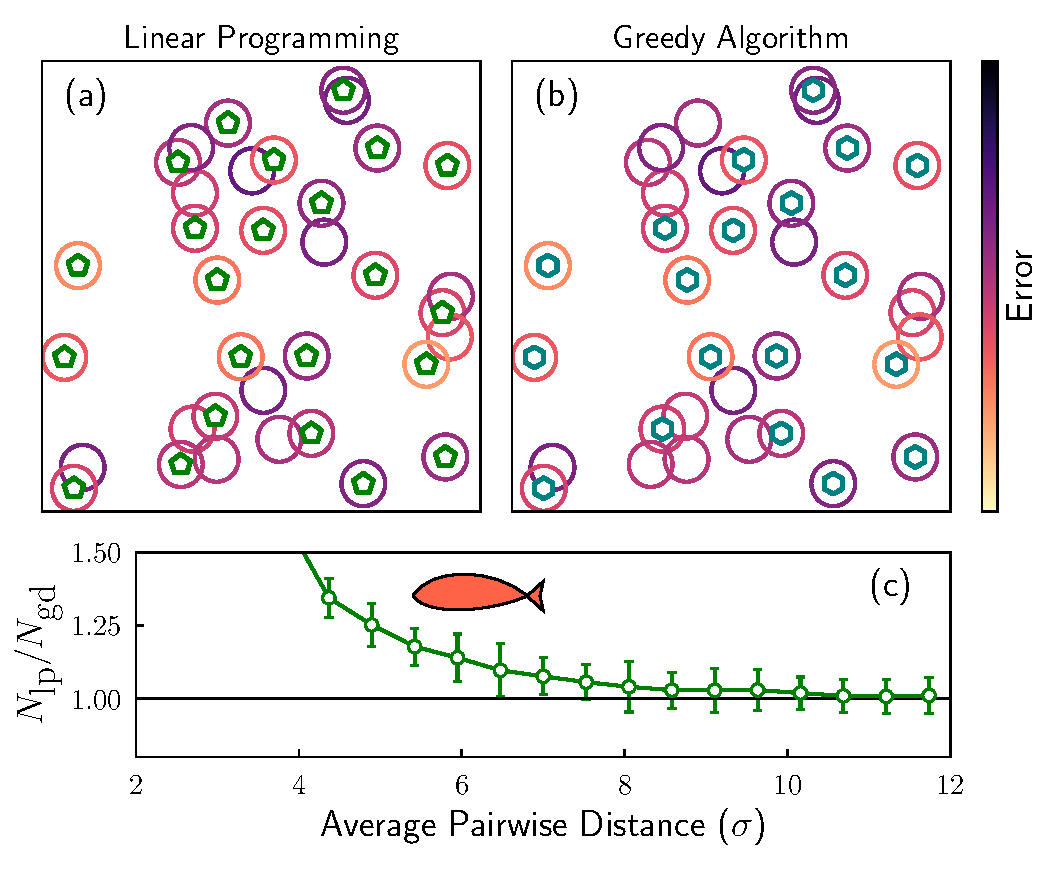
\includegraphics[width=\linewidth]{overlap}
  \caption[Removing the overlap particles with different algorithms]{
  The removal of overlapping particles with different algorithms. The circles represent particles. Their locations corresponds to $\{\mathbf{x}\}$, and their radius values are the hard core diameters ($\sigma$ in Eq.~\ref{eq:overlap}). The colour of the circles represents the error to be minimised.
  (a): the result of solving Eq.~\ref{eq:overlap}, implemented as algorithm~\ref{alg:overlap}. The pentagons represent the optimised result ($\{ \mathbf{x} \}_\textrm{opt}$).  
  (b): the result of greedy algorithm (algorithm~\ref{alg:overlap-greedy}). The hexagons represent the optimised result ($\{ \mathbf{x} \}_\textrm{opt}$).
  (c): the number ratio of optimised positions from algorithms~\ref{alg:overlap} ($N_\mathrm{lp}$) and algorithm~\ref{alg:overlap-greedy} ($N_\mathrm{gd}$) as a function of average pairwise. The positions were randomly sampled with different densities. The error bars were the standard error calculated from 25 different simulations.
  }
  \label{fig:overlap}
\end{SCfigure}


The systematic difference between the two algorithms is presented in Fig.~\ref{fig:overlap}(c). The ratio between the number of optimised particles, detected by different algorithms is plotted against the average pairwise distance of the particles. The linear programming method consistently generates larger optimised set, especially in the high density region, when the average pairwise distance is close to 2.
For the dilute system, the difference between the two algorithms were negligible. The average pairwise distance of zebrafish were close to 20 cm\cite{yang2021pcb,miller2007}, while the average body length of the fish was $\sim$ 3 cm. As a result, the fish is similar to the ideal gas particles where the average pairwise distance is close to 6 $\sigma$, where the difference between the two algorithms is significant. Because of its better performance, the linear programming method was selected to remove the overlapping particles. In the experiments, the size of the hard core was chosen to be 1 cm, a value that corresponds to the width of the fish.


\subsection{Removing Overlapping and \emph{Soft} Particles}

The overlap removing algorithm can be improved slightly, to change the strictly hard length scale ($\sigma$) to a ``softer'' counterpart. The idea was borrow from the soft margin classification problem for the support vector machine (SVM) algorithm in the machine learning (ML) community \cite{geron2019}. Following the naming tradition in ML literatures, we introduce a \emph{slack variable} $\zeta_{ij}$ for particle $i$ and $j$. The value of $\zeta_{ij}$ measures how soft the repelling is between two particles. The larger $\zeta_{ij}$ value corresponds to a softer particle. In the language of physics, the $\zeta_{ij}$ variables are essentially the pairwise potential energy between atoms, whose sum ($\sum_i\sum_j\zeta_{ij}$) gives the internal energy of a system, and should be minimised.

Formally, the overlap removing with soft interaction can be written down as follows,

\begin{equation}
\begin{aligned}
	\textrm{Minimize} && 
	\sum_i{(e_i + \mu) x_i} + \beta \sum_i \sum_j \zeta_{ij} \\
	\textrm{Subject to} &&  x_1 d_{12}  x_2 \le \sigma - \zeta_{12}\\
	&&  x_1 d_{13}  x_3 \le \sigma - \zeta_{13}\\
	&& \vdots  \\
	&& x_i d_{ij}  x_j \le \sigma - \zeta_{ij}
\label{eq:overlap-soft}
\end{aligned}
\end{equation}

\noindent which is a slight modification of Eq.~\ref{eq:overlap}.
Firstly, we remove the constraint that forces the total number of particles to equal $K$. 
There are also two additional parameters, \gls{mu} and \gls{beta}.
The parameter $\mu$ controls the number of total particles in $\{\mathbf{x}\}_\mathrm{opt}$. The smaller the $\mu$ value is, the more particles will be included in the optimised set. In the context of statistical mechanics, we can think of $\mu$ as the \emph{chemical potential}.
The parameter $\beta$ before the energy term $\sum_i\sum_j \zeta_{ij}$ controls the softness of the excluding zone around each coordinate, sharing the same meaning with the hyperparameter $C$ in the SVM algorithm. Within the context of statistical physics, the parameter $\beta$ is conceptually identical to the \emph{inverse temperature}. Reducing the value of $\beta$, we increase the temperature, and we make every particle appear softer. 

The solution of Eq.~\ref{eq:overlap-soft} will be identical to the solution of Eq.~\ref{eq:overlap}, when $\beta \rightarrow \infty$ and $\mu \sim -\max(\{ e_i \})$. These solutions were ascribed to the ``hard removal'' region in Fig.~\ref{fig:overlap-soft}(c). Fixing the value of $\mu$ but decrease $\beta$ gradually, move overlap will be allowed, and more particles will be detected. These regions were labelled as ``soft removal'' in Fig.~\ref{fig:overlap-soft}. When the values of both $\mu$ and $\beta$ were small, all the particles will be retained in $\{\mathbf{x}_\mathrm{opt}\}$, corresponding to the ``no removal'' region in Fig.~\ref{fig:overlap-soft}(c). On the other hand, the solution of Eq.~\ref{eq:overlap-soft} will lead to the removal of all particles, when the value of $\mu$ is large. This scenario corresponds to the ``excess removal'' region in Fig.~\ref{fig:overlap-soft}(c).


\begin{SCfigure}
  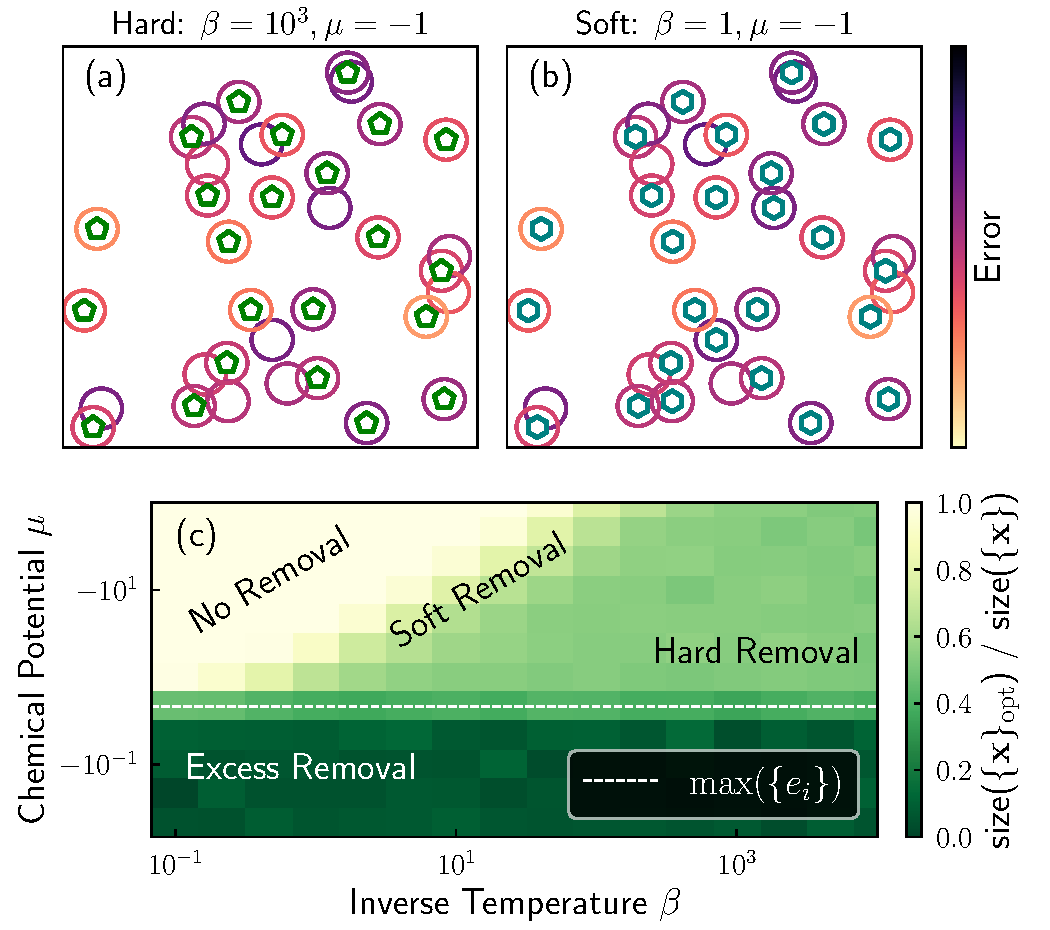
\includegraphics[width=\linewidth]{overlap-soft}
  \caption[Removing the overlap particles with soft constraint]{
  The removal of overlapping particles following equation~\ref{eq:overlap-soft}. The circles represent particles ($\{\mathbf{x}\}$). The colour of the circles represent their errors.
  (a): the result with parameters $\beta=10^3$ and $\mu=-1$. The pentagons represent the optimised result ($\{ \mathbf{x} \}_\textrm{opt}$). The result is identical to that in Fig.~\ref{fig:overlap}.
  (b): the result with parameters $\beta=1$ and $\mu=-1$. The pentagons represent the optimised result ($\{ \mathbf{x} \}_\textrm{opt}$).
  (c): the ratio between the number of particles after and before the optimisation, as a function of the two parameters. The $x$ axis corresponds to the inverse temperature $\beta$, and the $y$ axis corresponds to the chemical potential $\mu$. Different regions were labelled with their characteristic behaviour. The dashed line shows the maximum value of the error. Each grid in (c) represents the average of 25 ideal-gas simulations.
  }
  \label{fig:overlap-soft}
\end{SCfigure}


This soft overlap-removal algorithm was implemented, but not tested nor used for the fish data. This is because the determination of the parameters, $\mu$ and $\beta$, is difficult. However, this soft overlap remove algorithm presents as a promising algorithm for the real-space colloidal microscopy, as the energy term can take realistic, inter-colloidal interaction form, to match the experimental system.

\section{From Better Locations to Trajectories}
\label{section:link}

The overlap-free positions can be linked into trajectories, from which we can get the velocities of the fish. The term ``link'' means finding the fish $j$ at time $t+1$, which corresponds to the fish $i$ at time $t$, and the pair $(i, j)$ forms a link.
Such a linking process therefore gives us the identity of each fish in different time points.
The movement of a single fish, as a function of time, forms a \emph{trajectory}.
The process of linking coordinates into trajectories is commonly applied in different fields, for instance in the analysis of colloidal experiments\cite{crocker1996} as well as fluid dynamic experiments\cite{ouellette2005ef}.


Two examples of the linking process are illustrated in Fig.~\ref{fig:link-idea}, where the locations of 6 simulated fish in 3 successive frames were linked into 6 trajectories. The good links were illustrated in Fig.~\ref{fig:link-idea}(a) while the poor links were shown in Fig.~\ref{fig:link-idea}(b).
Visually, the trajectories in (b) were poor because the resulting trajectories contain sudden jumps between different locations. Intuitively, we would not expect the fish to jump back and forth from place to place.

The method of linking experimental coordinates of animals into trajectories always involves some ``educated guesses''. This is because we do not know the underline dynamics of the animals that we were studying, as we could not predict precisely where the animal will move to from its past trajectory. In this section, two heuristic methods that ``worked'' will be introduced.


\subsection{Equilibrium Linking}
\label{section:link-eq}


With the observation in Fig.~\ref{fig:link-idea}, it is reasonable to assume that the links yielding smallest total movement for all the fish, are good links. Formally, our linking procedure will aim at minimising the total squared movement \gls{tsm}, which is written as 

$$
\Delta = \sum_i\sum_t\delta_i(t)^2,
$$

\noindent where $i$ corresponds to all the linked trajectories, and $\delta_i(t)$ is the distance that a fish travelled between time $t-1$ and $t$. In fact, \citeauthor{crocker1996} showed that the minimisation of $\Delta$ is equivalent to maximising the probability, if the fish were non-interacting diffusive Brownian particles in equilibrium \cite{crocker1996}.
Even though the underlying assumption is crude, this method produces visually good trajectories for fish.
The linking algorithm that minimises $\Delta$ is termed as \emph{equilibrium linking}, since it is suitable for physical systems in equilibrium.


\begin{SCfigure}
  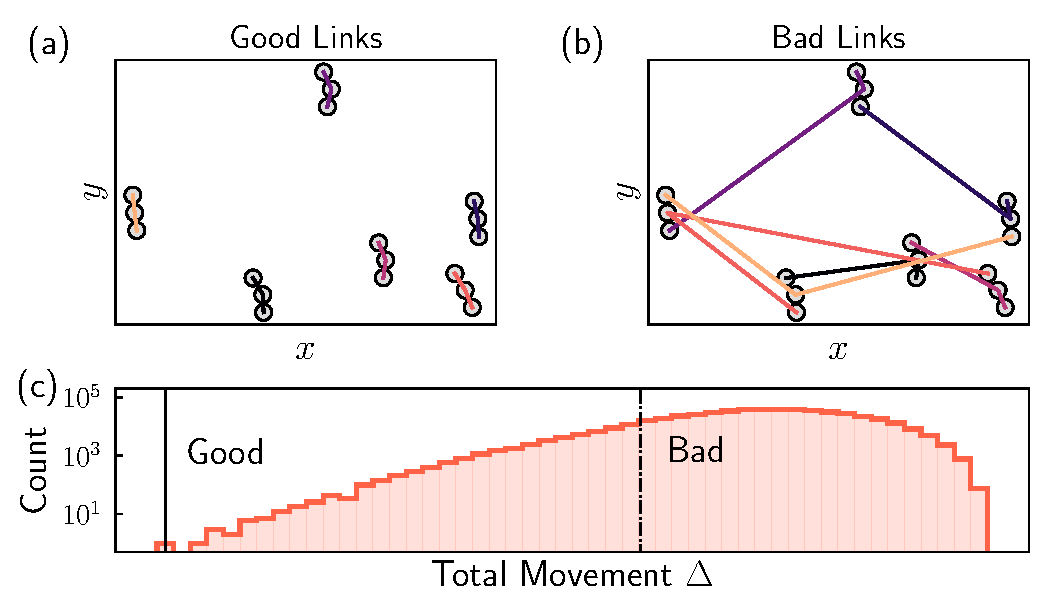
\includegraphics[width=\linewidth]{linking-idea}
  \caption[Linking locations into trajectories: concept illustration]{
  (a): the good way to link positions in 3 successive frames into trajectories.
  (b): the bad way to link positions in 3 successive frames into trajectories.
  (c): The distribution of total movement ($\Delta$) for all the possible linking options ($6!^2=518,400$ possibilities). The good linking result corresponds to the links that yields the minimum of $\Delta$.
  }
  \label{fig:link-idea}
\end{SCfigure}


Unfortunately, the minimisation of \gls{tsm} is a difficult task. Naively, we may attempt to list all the possible links, and choose the one with minimum $\Delta$ value as our linking result. However, the complexity of this approach is $\mathcal{O}((N!)^{T-1})$ \cite{crocker1996}, where $N$ is the number of fish, and $T$ is the total number of time points. For the experiment with 10 fish in 20 total frames, we need to enumerate $\sim 10^{130}$ possible combinations, which is not practical.\marginfootnote{
	To find the minimum number in an array with size of $10^{130}$, we need $\sim 10^{103}$ years, using a laptop with infinite memory. People die in the timescale of $\sim 10^2$ years.
}

To reduce the complexity, we restrain the particles to have a maximum movement between two frames \cite{crocker1996}, and analyse the data frame-by-frame, rather than optimise the entire trajectory. A good implementation of this approach is available in the \code{Trackpy} package \cite{allan2021}. Unavoidably, the introduction of extra assumptions will deviate the obtained solution, the linked trajectories, away from the true global minimum of $\Delta$. And even with the reduced complexity, the equilibrium linking algorithm can be extremely slow, when multiple equally good linking options being available.

\subsection{Active Linking}
\label{section:link-act}

\begin{SCfigure}
  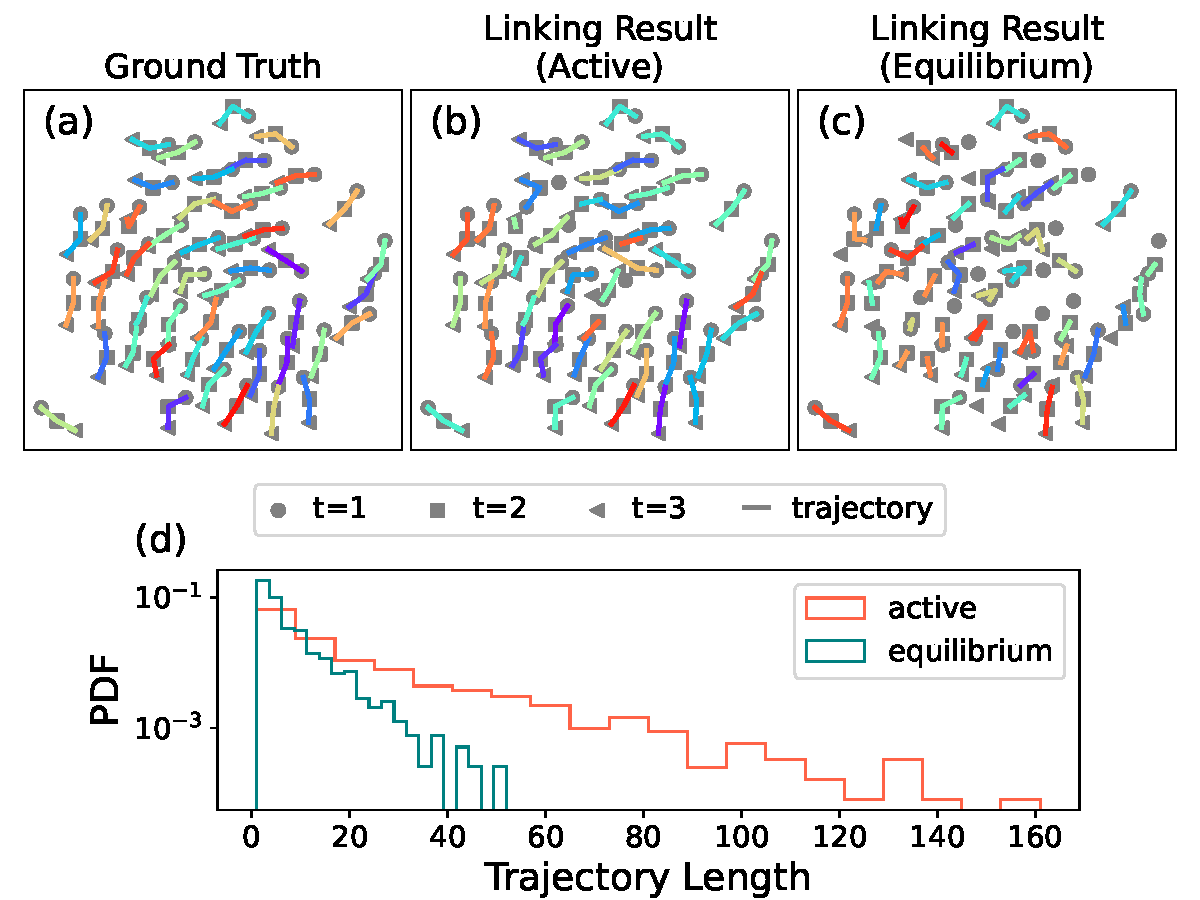
\includegraphics[width=\linewidth]{linking-sim}
  \caption[Comparing two linking algorithms]{
  The linking process to get trajectories from positions. The grey solid scatters represents the location ($\{\mathbf{x}\}$) of simulated particles. The coloured lines represent the linked trajectories. Some positions were discarded (rendered as empty scatters) randomly to mimic the experimental locations.
  (a) The ground truth.
  (b) The result with the active linking algorithm.
  (c) the result with the equilibrium linking algorithm.
  (d) The distribution of trajectory length values for different linking algorithms. Better algorithms are expected to produce longer trajectories.
  }
  \label{fig:link-sim}
\end{SCfigure}

For systems that are out of equilibrium, like a school of fish, the assumption introduced in section~\ref{section:link-eq} is not formally correct. In this project, another good heuristic approach proposed by \citeauthor{ouellette2005ef} was used to link the coordinates \cite{ouellette2005ef}.
For particle $i$ at time $t$ and particle $j$ at time $t+1$, the link $(i, j)$ was established by minimising the \emph{tracking cost},

$$
\phi_{ij}^{t} = \left\Vert
\mathbf{x}_j^{t+2} - \hat{\mathbf{x}}_i^{t+2}
\right\Vert,
$$

\noindent where $\mathbf{x}_j^{t+2}$ is the location of particle $j$ in time point $t + 2$, and $\hat{\mathbf{x}}_i^{t+2}$ is the predicted location of particle $i$ in time point $t + 2$. The prediction was calculated with the following

$$
\begin{aligned}
\hat{\mathbf{x}}_i^{t + 2} &= 
\mathbf{x}_i^t + 
\mathbf{v}_i^t + 
2 \mathbf{a}_i^t = 
3 \mathbf{x}_i^{t+1} - 
3 \mathbf{x}_i^t +
\mathbf{x}_i^{t-1} \\
\mathbf{v}_i^t &= (\mathbf{x}_i^{t+1} - \mathbf{x}_i^{t - 1}) / 2 \\
\mathbf{a}_i^t &= 
\mathbf{x}_i^{t+1} - 2 \mathbf{x}_i^{t} + \mathbf{x}_i^{t-1}.
\end{aligned}
$$

\noindent In reference~\cite{ouellette2005ef} this method was named as the four frame best estimate method. Operationally, for particle $i$ in time point $t$, we search for all the possible particle $j$ in time point $t+1$, and establish link with the minimum $\phi_{ij}^t$, by predicting the location of the trajectory with link $(i, j)$ in time point $t + 2$. This linking method is noted as the \emph{active} linking method.

The behaviour of the two linking methods was exhibited in Fig.~\ref{fig:link-sim}, where simulated trajectories were used for the test. The model used in the simulation is the inertial Vicsek model, which will be introduced in chapter~\ref{chapter:fish_model}. The model generates trajectories that are similar to that of the zebrafish, and the generated coordinates were used to test the different linking algorithm.
Both methods generated visually good trajectories.
However, the equilibrium linking method obtain shorter trajectories, as shown in Fig.~\ref{fig:link-sim}, which indicates that the behaviour of the equilibrium linking method is poor. For all the fish data, the active linking method was used.



\subsection{Extending the Trajectories}

The linking algorithms typically give us some short trajectory segments. These segments can be extended further following \citeauthor{xu2008}'s method. The idea is to join the two trajectories together, if the the prediction from earlier trajectory matched the locations of the later trajectory \cite{xu2008}.

The result of the relinking method is illustrated in Fig.~\ref{fig:relink}. The coordinates to be linked and relinked was generated from simulation, where 25 simulated agents were performing a U-turn together. Some of the coordinates (2\%) were deliberately removed during linking, in order to mimic the various locating errors in reality. 

For perfect coordinates, the active linking method was capable of obtaining correct trajectories. However, the introduction of missing particles makes this linking process problematic. As illustrated in Fig.~\ref{fig:relink}(a), many short trajectory segments were obtained. The relinking process successfully re-joined these segments into very long trajectories, as shown in Fig.~\ref{fig:relink}(b). The relinked trajectories were very long, and half of them have the full length, as shown in Fig.~\ref{fig:relink}(c). For the experimental fish coordinates, the relinking process is valuable, as it always extends the short trajectories (from the active linking method) into longer ones.


\begin{SCfigure}
  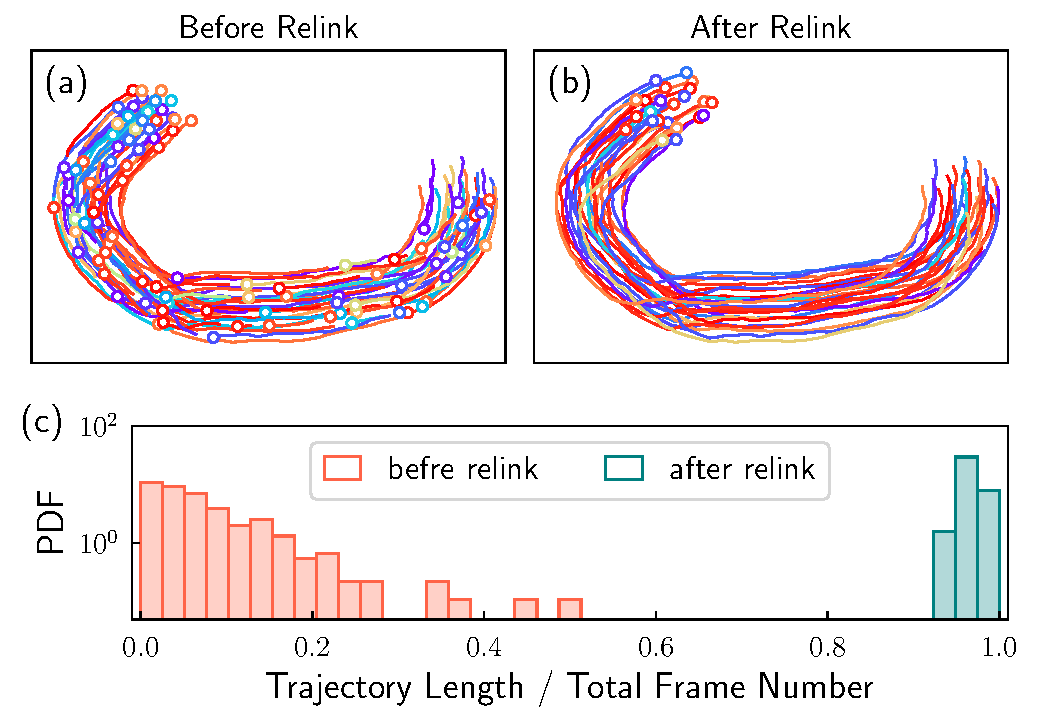
\includegraphics[width=\linewidth]{relink}
  \caption[The effect of relinking]{
  	The effect of relinking process with simulated data.
  	(a) The trajectories linked with the active linking method.
  	(b) The trajectories extended with the relinking method.
  	(c) The distribution of the trajectory length. The length values were rescaled by the total frame number. The trajectory with length value being close to 1 corresponds to a full trajectory through out the entire simulation.
  }
  \label{fig:relink}
\end{SCfigure}


\section{From Trajectories to Behaviour}
\label{section:trajectory-analysis}

The trajectories contain rich information about the behaviour of the zebrafish.
The analysis to reveal the behaviour of the fish will be discussed in this section.
For the structure of the fish group, we introduce the nearest neighbour distance, the convex hull, and the radial distribution function, as different characterisation tools. On the other hand, the average speed, the orientational relaxation time, the polarisation order and the persistence length will be discussed as the quantities to describe the dynamics of the fish.


\subsection{The Structure}

The coordinates of the fish shed light on the the \emph{structure} of the group, giving answers to the following questions.

\begin{enumerate}
	\item How close do a pair of fish stay to each other?
	\item How big is the animal group in terms of the metric size?
	\item Are the fish arranged in an ordered way (like atoms in a crystal) or a disordered way (like atoms in a fluid phase)?
\end{enumerate}

To answer the first question, we can calculate the nearest neighbour distance of the fish, whose usage could be traced back to 1960s \cite{cullen1965}. The average nearest neighbour distance of fish (\gls{lnn}) is defined as,

\begin{equation}
	l_\textrm{nn} =\frac{1}{N}\sum_i\min_{j (\neq i)}(d_{ij})
\label{eq:nnd}
\end{equation}

\noindent where \gls{dij} is the pairwise distance of fish $i$ and $j$, and $N$ is the total amount of fish. The average nearest neighbour distance of a group could serve as a measure of the cohesiveness of the fish. The group with smaller $l_\textrm{nn}$ value appear more cohesive.

To measure the size of the group, we can measure area (for 2D data) or the volume (for 3D data) of the \emph{convex hull}, constructed from the coordinates of the fish. The convex hull is the smallest subset of the space, which contains all line segments connected by all pairs of points \cite{berg2000}. Intuitively, the convex hull is the smallest polygon (or polyhedron for 3D coordinates) that encloses all coordinates. An example of the convex hull constructed from 50 fish were provided in Fig.~\ref{fig:structure-2d}(a). The area ($A_\mathrm{ch}$) or the volume ($V_\mathrm{ch}$) of the hull can be transformed into a lengthscale\marginfootnote{
To describe the completely geometry of the group, we need to consider more details, since a group of fish does not always present the shape of a sphere. These extra details include the aspect ratio, or the thickness. By assuming the group shape to be spherical, we can use just one number to describe it. Such simplified description can be thought of as a first order approximation.
}, termed as the \emph{effective convex hull diameter} \gls{lch}, which is defined as

\begin{equation}
\begin{split}
	l_\mathrm{ch}
	&= \left(
	\frac{4}{\pi} A_\mathrm{ch}
	\right)^\frac12 (\mathrm{2D}\ \mathrm{Coordinates}) \\[1.5ex]
	&= \left(
	\frac{6}{\pi} V_\mathrm{ch}
	\right)^\frac13 (\mathrm{3D}\ \mathrm{Coordinates}),
\end{split}
\label{eq:convex-hull-diameter}
\end{equation}

\noindent where the shape of the convex hull were assumed to be circular (for 2D coordinates) or spherical (for 3D coordinates). The effective convex hull diameter is a measure of the group size.

Both lengthscales, the effective convex hull diameter and the nearest neighbour distance, capture the cohesiveness of the group. In fact, they were often linearly correlated for the zebrafish, as shown in Fig.~\ref{fig:nnd-ch-corr}. Therefore, we only need one of them to describe the fish behaviour. The nearest neighbour distance was selected, because it is more widely used in the past.

\marginpar{
\centering
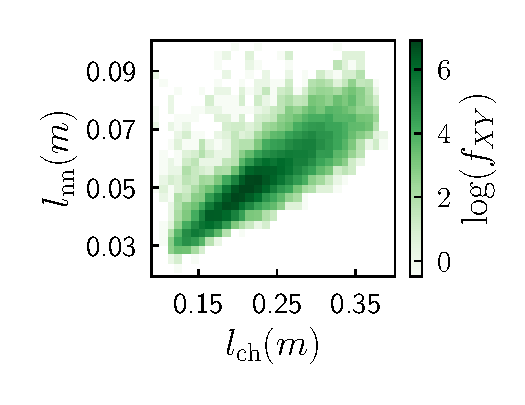
\includegraphics[width=\marginparwidth]{nnd-ch-corr}
\captionof{figure}{The joint probability density function ($f_{XY}$) of $l_\mathrm{nn}$ and $l_\mathrm{ch}$. The results were obtained from 3D experimental data of 50 adult zebrafish.}
\label{fig:nnd-ch-corr}
}


Finally, we can calculate the radial distribution function (the $g(r)$) of the fish to inspect whether the structure of the fish was ordered or not. However, the spatial distribution of a group of fish may not be homogeneous in the experiment, possibly being affected by environmental factors such as the distribution of brightness, as shown in the results in chapters~\ref{chapter:fish_2d} and \ref{chapter:fish_3d}. Therefore, the pairwise distances ($\{ d_{ij} \}$) would be biased to favour the lengthscale of the high density region. In other words, the fish appear to swim together. But they were driven by an external field, instead of being attractive to each other.

To remedy the effect of the external field, we can compare the pairwise distances of the fish $\{d_{ij}\}^\textrm{fish}$ to the pairwise distances of the ideal gas particles $\{d_{ij}\}^\textrm{gas}$, that share the same inhomogeneous spatial distribution with the fish.
Operationally, we calculate the density distribution of the fish, and sample ideal gas particles drawn randomly from the same density distribution, using the tower-sampling method \cite{krauth2006}.
Therefore, the sampling of the ideal gas particles is biased, in contrast to a uniform distribution in the boundary. The biased sampling result was illustrated in Fig.~\ref{fig:structure-2d}(a) and Fig.~\ref{fig:structure-3d}(a), where the distribution of the ideal gas is identical to that of the fish.


Even though the biased ideal gas particles share the same density distribution with the fish, these two systems are inherently different. The ideal gas particles do not interact with each other, but the fish do.
Such a difference will lead to different pairwise distances, whose probability density function was noted as \gls{pdfd}.
For instance, we can not imagine two fish with a separation of zero, as the fish can not physically overlap.
Such a repulsive interaction will decrease the likelihood of finding two fish at very short distances.
 
The ratio between the $f_d(r)$ from the fish and the ideal gas, was defined as the radial distribution function, \gls{gr}:

\begin{equation}
	g(r) = \frac{f_d^\textrm{fish}(r)}{f_d^\textrm{gas}(r)}.
\label{eq:gr}
\end{equation}

\noindent The value of $g(r)$ indicates the likelihood of finding a pair of fish at the distance $r$, with respect to the ideal gas particles. When $g(r)$ is equal to one, it is equally likely to find a pair of fish or to find a pair of ideal gas particles, indicating the lack of correlation. When the value of $g(r)$ is greater than one, the density of the fish correlates positively, suggesting a cohesive behaviour.

For the structure of dilute liquid, we often get a peak in the $g(r)$, followed by a monotonic decay. The location of the peak is often close the $l_\mathrm{nn}$. The subsequent decay revealed another lengthscale, which was termed the correlation length of the density ($\xi_\rho$). The definition of \gls{xirho} is

\begin{equation}
	g(\xi_\rho) = 1; (\xi_\rho > l_\mathrm{nn}).
\label{eq:length-density}
\end{equation}

\noindent and we force the value of $\xi_\rho$ to be greater than $l_\mathrm{nn}$, effectively removing the situation where $g(r)$ reaches zero at very small distance values.

In addition to the lengthscales, the height of the peak of $g(r)$ give us a measure of the cohesiveness of the group. Inspired by liquid state theory, we define the logarithm of the peak value of $g(r)$ as the \emph{effective attraction} \gls{attr} \cite{hansen2013}:

\begin{equation}
\epsilon = -\log\left(
	\max(g(r))
\right).
\label{eq:effective-attraction}
\end{equation}

\noindent The quantity $\epsilon$ is a better measure of the cohesion of the fish, because it could differentiate whether the fish is cohesive or not. For a non-cohesive group, the value of the $g(r)$ will be close to one, leading a value of 0 for $\epsilon$. The lack of cohesion could be be identified by the lengthscales.


\begin{table}
\begin{adjustwidth*}{0in}{-1.5in}
	\centering
	\begin{tabular}{ l l c c l }
		\toprule
		Symbol & Definition & Value (2D) & Value (3D) & Meaning\\
		\midrule
		$l_\mathrm{nn}$ &
		Eq.~\ref{eq:nnd} &
		61 $\pm$ 10 mm &
		51 $\pm$ 10 mm &
		Nearest Neighbour Distance
		\\
		$l_\mathrm{ch}$ &
		Eq.~\ref{eq:convex-hull-diameter} &
		0.8 $\pm$ 0.46 m &
		0.29 $\pm$ 0.25 m &
		Convex Hull Diameter\\
		$l_p$ &
		Eq.~\ref{eq:lp} &
		$\sim 0.13$ m &
		$\sim 0.14$ m &
		Persistence Length\\
		$\xi_\rho$ &
		Eq.~\ref{eq:length-density} &
		$\sim 0.4$ m &
		$\sim 0.32$ m &
		Correlation Length of the Density\\
		$\xi_v$ &
		Eq.~\ref{eq:length-dynamics} &
		$\sim 0.15$ m &
		$\sim 0.12$ m &
		Correlation Length of the Speed\\
		$\xi_\mathbf{o}$ &
		Eq.~\ref{eq:length-dynamics} &
		$\sim 0.38$ m &
		$\sim 0.24$ m &
		Correlation Length of the Orientation\\
		$\tau_\mathbf{o}$ &
		Eq.~\ref{eq:tau} &
		$\sim 1.3$ s &
		$\sim 0.9$ s &
		Relaxation Time of the Orientation\\
		$\tau_\rho$ &
		Eq.~\ref{eq:tau} &
		$\sim 900$ s &
		$\sim 180$ s &
		Relaxation Time of the Density\\
	\bottomrule
	\end{tabular}
\caption{
Different Length Scales and Time Scales for 50 Zebrafish.}
\label{table:behaviour}
\end{adjustwidth*}
\end{table}

\subsection{The Dynamics}

The velocities can be calculated as the time derivative of the positions along the trajectories, once we linked the coordinates. The velocities offered the \emph{dynamics} of the system, giving answers to the following questions.

\begin{enumerate}
	\item How fast do the fish swim?
	\item Is the movement of the fish ordered or random?
	\item How long does it take for the fish group to forget its current state?
\end{enumerate}

To answer the first question, we could simple calculate the average speed of the fish, which is defined as,

\begin{equation}
	v = \frac1N \sum_i{\left\Vert \mathbf{v}_i \right\Vert},
\label{eq:speed}
\end{equation}

\noindent where the $\mathbf{v}_i$ is the location of fish $i$, and $N$ is the total amount of the fish. With higher \gls{spd} value, the animals on average move faster.
The distribution of the average speed of 50 zebrafish in 3D was shown in Fig.~\ref{fig:dynamics-3d}(a).

Being conceptually similar to the average speed, the speed of the entire group can be calculated as,

$$
v_g = \frac1N \left\Vert
\; \sum_i{\mathbf{v}_i} \;
\right\Vert.
$$

\noindent This quantity indicates the speed of the group centre. A large group speed value indicates the fish  moving collectively from one place to another. Formally, we define an \emph{order parameter} to describe such behaviour, by modifying the group speed:

\begin{equation}
	\Phi = \frac1N \left\Vert
		\; \sum_i \mathbf{o}_i \;
	\right\Vert
	= \frac1N \left\Vert
		\sum_i \frac{\mathbf{v}_i}{\Vert \mathbf{v}_i \Vert}
	\right\Vert,
\label{eq:polarisation}
\end{equation}

\noindent where \gls{pol} is called the \emph{polarisation}\marginfootnote{
	The polarisation is conceptually similar to the magnetisation per spin in the Ising model. When the order parameter approaches one, the system is ordered.
	The polarisation is identical to the magnetisation defined in XY model (in 2D) and Heisenberg model (in 3D), when the orientations of the fish was treated as the spin vectors \cite{newman1999}.
}, and $\mathbf{o}_i$ is the orientation of fish $i$. The definition of $\Phi$ ensures it varies from 0 to 1, like other order parameters in statistical mechanics.
The movement of a group of fish is ordered if the value of $\Phi \sim 1$, and the movement being disordered when $\Phi \sim 0$.


For a group of fish, their structural quantities ($l_\mathrm{nn}, l_\mathrm{ch}, g(r)$) and their dynamic quantities ($v, \Phi$) change constantly. With the \emph{time-displaced autocorrelation function} (ACF) of these quantities, we can probe the typical timescale for the fluctuation of these quantities. The ACF of quantity \gls{cat} is defined as, \cite{newman1999}

\begin{equation}
\begin{split}
	C_\mathcal{A}(t)
	&= \int d\tau
	\left(
		\mathcal{A}(\tau) - \bar{\mathcal{A}}
	\right)
	\left(
		\mathcal{A}(\tau + t) - \bar{\mathcal{A}}
	\right) \\
	&= \langle \mathcal{A}(t) \mathcal{A}(t + \tau) \rangle.
\label{eq:acf}
\end{split}
\end{equation}

\noindent where $\bar{\mathcal{A}}$ is the time-average $\mathcal{A}$. For the ACF of the orientation of the fish, the shape of \gls{cot} exhibits a typical exponential decay. Such ACF was commonly obtained from the Markov processes, where the $C_\mathcal{A}(t)$ could be written as a sum of exponential functions,

\begin{equation}
\begin{split}
	C_\mathcal{A}(t) &= \sum_i \left( a_i \exp{-t / \tau_i} \right)\\
	&\sim \exp\left(-t / \tau\right).
\end{split}
\label{eq:tau}
\end{equation}

\noindent Here the shape of $C_\mathcal{A}$ is often dominated by the largest time scale ($\tau$).\marginfootnote{
This timescale corresponds to the second largest eigenvector of the transition matrix of the Markov process.
}
Therefore, we define the timescale when $C_\mathbf{o}$ reaches $1/e$ as the relaxation time orientation, noted as $\tau_\mathbf{o}$. For other quantities, the shapes of their corresponding $C_\mathcal{A}(t)$ functions are complicated. We therefore define the time when their corresponding $C_\mathcal{A}(t)$ reach zero as their relaxation time scales.

Regardless of the slightly different definition, the value of the relaxation time \gls{taua} indicates the time taken for a system to forget its current state.
For instance, the value of $\tau_\mathrm{nn}$ is the time for a group fish to forget their nearest neighbour distance. Because the two density-related quantities, $l_\mathrm{nn}$ and $l_\mathrm{ch}$, are strongly correlated, their corresponding ACFs ($C_\mathrm{nn}(t)$ and $C_\mathrm{ch}(t)$) are also very similar. Therefore, we term their relaxation time as the relaxation time of density, written as $\tau_\rho$. The examples of relaxation time scales for the orientation and density are available in Table~\ref{table:behaviour}. Practically, these two time scales are the only dominating time scales for the fish, in all of our observations.


In addition to the timescale of the structural quantities, we could also calculate the lengthscale of the dynamical quantities. For instance, we can take the the product of the average speed $v$ (Eq.~\ref{eq:speed}) and the orientation relaxation time $\tau_\mathbf{o}$ (Eq.~\ref{eq:tau}), as the \emph{persistence length}:

\begin{equation}
	l_p = v \ \tau_\mathbf{o}.
\label{eq:lp}
\end{equation}

\noindent The value of \gls{lp} corresponds to the distance that a fish travels in a straight fashion. For the fish with a small $l_p$ value, its trajectory appear more curvy. 

In addition to the persistence length, we can also measure the correlation length of the dynamics of the fish. If a fish changed its speed at a certain time point, it is interesting to know how far would such change reach. To do so, we calculate the \emph{connected correlation function} of the dynamical quantities \cite{newman1999, cavagna2014}\marginfootnote{
	The correlation function $C_\mathcal{A}(r)$ with variable ``$r$'' is a spatial correlation function, which gives us a correlation length $\xi_\mathcal{A}$. The correlation function $C_\mathcal{A}(t)$ with variable ``$t$'' is a temporal correlation function, which gives us a relaxation time $\tau_\mathcal{A}$.
}:

\begin{equation}
\begin{split}
	C_{\mathcal{A}}(r) 
	&= \iint d\mathbf{r} d\mathbf{r^\prime} \;
	\left(
		\mathcal{A}(\mathbf{r}) - \bar{\mathcal{A}}
	\right)
	\left(
		\mathcal{A}(\mathbf{r} + \mathbf{r^\prime}) - \bar{\mathcal{A}}
	\right)
	\delta(\Vert \mathbf{r} - \mathbf{r^\prime} \Vert - r) \\[2ex]
	&= \frac{\sum_i\sum_{j \neq i}
		\left[
			(\mathcal{A}_i - \bar{\mathcal{A}})
			(\mathcal{A}_j - \bar{\mathcal{A}})
			\delta(r - r_{ij})
		\right]
	}
	{\sum_i\sum_{j \neq i} \delta(r - r_{ij})}
\label{eq:cr}
\end{split}
\end{equation}

\noindent where $\delta(r - r_{ij}) = 1$ when $r = r_{ij}$, and it equals zeros otherwise. The correlation functions often exhibits a monotonic decay when $r > l_\mathrm{nn}$. We define the length when the correlation function $C_\mathcal{A}(r)$ reaches zero as the \emph{correlation length} of $\mathcal{A}$:

\begin{equation}
	C_{\mathcal{A}}(\xi_\mathcal{A}) = 0.
\label{eq:length-dynamics}
\end{equation}


\noindent The examples of the correlation functions for the speed \gls{cvr} and for the orientation \gls{cor} were shown in Fig.~\ref{fig:dynamics-2d}(e) and Fig.~\ref{fig:dynamics-3d}(e).

%Figure~\ref{fig:dynamics} (e) shows the correlation function for the orientation ($C_\mathbf{o}(r)$) and the speed ($C_{v}(r)$) from 50 zebrafish. It is obvious that these quantities exhibits different length-scales.

%Then we obtain $l_\mathbf{o} \sim 0.2m$, and $l_v \sim 0.1 m$. This indicates that the orientation of the fish would affect neighbours further away, than the speed of the fish. This might be the reason that the fish do not form a coherent, flocking group like the birds, as they do not synchronise their speed effectively. In addition, the correlation length of the orientation, $l_\mathbf{o}$, is smaller than the effective convex hull diameter ($l_\mathrm{cm}$) of the fish. This is similar to the correlation length of midges in the laboratory \cite{vandervaart2020}.



\section{The Behaviour of 50 Zebrafish in 2D}

The coordinates of 50 zebrafish in a quasi-2D experiment, obtained with the methods introduced in chapter~\ref{chapter:fish_2d}, were linked into trajectories, from which the behaviour of these fish were analysed. The result for such experiment will be introduced in this section.

\subsection{The Structure}
\label{section:analysis-structure-2d}


The structure of 50 zebrafish was shown in Fig.~\ref{fig:structure-2d}. The spatial distribution was presented in Fig.~\ref{fig:structure-2d}(a), which was used to sample the biased ideal gas particles. The distribution of the pairwise distance, $f_d(r)$, was presented in Fig.~\ref{fig:structure-2d}(b). It is obvious the fish were more cohesive than the ideal gas particles, indicated by the mode of the distribution of the pairwise distances. The ratio of these distributions gives the $g(r)$ of the fish (Eq.~\ref{eq:gr}), which is shown in Fig~\ref{fig:structure-2d} (c). The distribution of $l_\mathrm{nn}$ and $l_\mathrm{ch}$ are presented in Fig~\ref{fig:structure-2d} (d).

The important structural feature revealed in Fig~\ref{fig:structure-2d} is the separation of $\xi_\rho$ and $l_\mathrm{ch}$, as the effective convex hull diameter ($l_\mathrm{ch}$, Eq.~\ref{eq:convex-hull-diameter}) is much larger than the correlation length of the density ($\xi_\rho$, Eq.~\ref{eq:length-density}).
This corresponds to the fragmentation of the fish group, where the 50 fish separated into sub-clusters. This scenario was plotted in Fig.~\ref{fig:structure-2d}(a), where the locations of the fish were represented as cross markers. There are clearly two dense blobs within the convex hull. And the size of these dense blobs is accurately captured by $\xi_\rho$.

As a consequence of the monotonic decay in $g(r)$, the fish group present a void at larger separation distances, where the value of $g(r) < 1$, shown in Fig.~\ref{fig:structure-2d}(a). As a result of the fragmentation of the fish group, the void also appear inside the fish group. The fragmentation of the fish group could explain the very wide distribution of $l_\mathrm{ch}$ observed in Fig.~\ref{fig:structure-2d}(d). If two sub-groups meet, the entire group will have a small value for its $l_\mathrm{ch}$. If the sub-groups were separated, the fish will exhibit a large $l_\mathrm{ch}$ value. 


 \begin{SCfigure}
  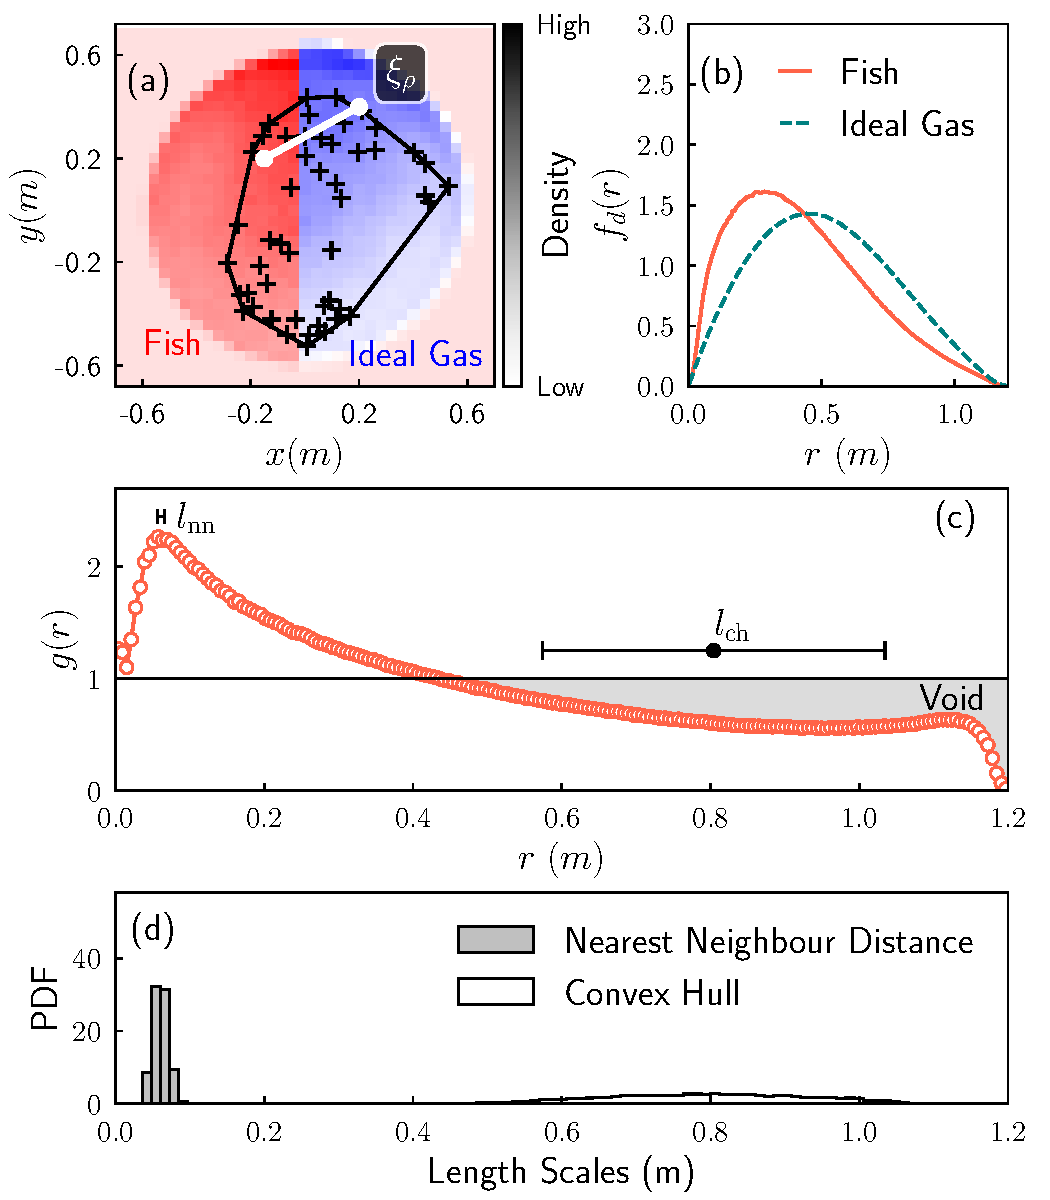
\includegraphics[width=\linewidth]{structure-2d-50}
  \caption[The structure of 50 zebrafish in 2D]{
  The structure of 50 zebrafish in a quasi-2D experiment.
  	(a) The joint distribution of the $x$ and $y$ coordinates of the fish and the ideal gas particles. The distribution of the ideal gas were biased to be identical to the fish. The location of 50 fish at one time point were plotted as circles. The boundary convex hull of these 50 scatters were plotted as solid lines.
  	(b) The probability density function of the pairwise distributions for the fish and the ideal gas particles in 2D.
  	(c) The radial distribution function, $g(r)$ (Eq.~\ref{eq:gr}) of the fish. It is defined as the ratio between the two PDFs in (b). Two important length scales, the nearest neighbour distance and the size of the convex hull were captured by the $g(r)$. The long distance region where $g(r) < 1$ corresponds to the void in the tank, where the group were able to explore.
  	(d) The distribution of the nearest neighbour distance and the effective diameter of the convex hull, of the fish.
  }
  \label{fig:structure-2d}
\end{SCfigure}

\subsection{The Dynamics}

The dynamics of the 50 fish are shown in Fig.~\ref{fig:dynamics-2d}. Figure~\ref{fig:dynamics-2d} (a) - (c) shows the distribution of the polarisation $\Phi$ (Eq.~\ref{eq:polarisation}) and the average speed $v$ (Eq.~\ref{eq:speed}). Their joint distribution appear to be very weakly correlated, as exhibited in Fig.~\ref{fig:dynamics-2d}(b). Overall, the fish were in a random state where $\Phi \sim 0.25$.



The ACFs (Eq.~\ref{eq:acf}) of different quantities were shown in Fig.~\ref{fig:dynamics-2d}(d). Two well separated time scales could be identified from these functions. For the time scale of $\sim$ 1s, the fish changed its orientation, and the value of $C_\mathbf{o}(t)$ decays to $1/e$. This timescale also dominates the ACF of the polarisation ($C_\Phi(t)$). 

Ones possible explanation for this observation, is to assign an intrinsic orientational diffusion constant for the fish. In other words, we assume the fish will sporadically change its swimming direction every now and then. And these random change makes the fish forget its original orientation, in the timescale of one second. Since the orientational diffusion is an inherent property of the fish, it would affect the collective order ($\Phi$) of a fish group.

\begin{SCfigure}
  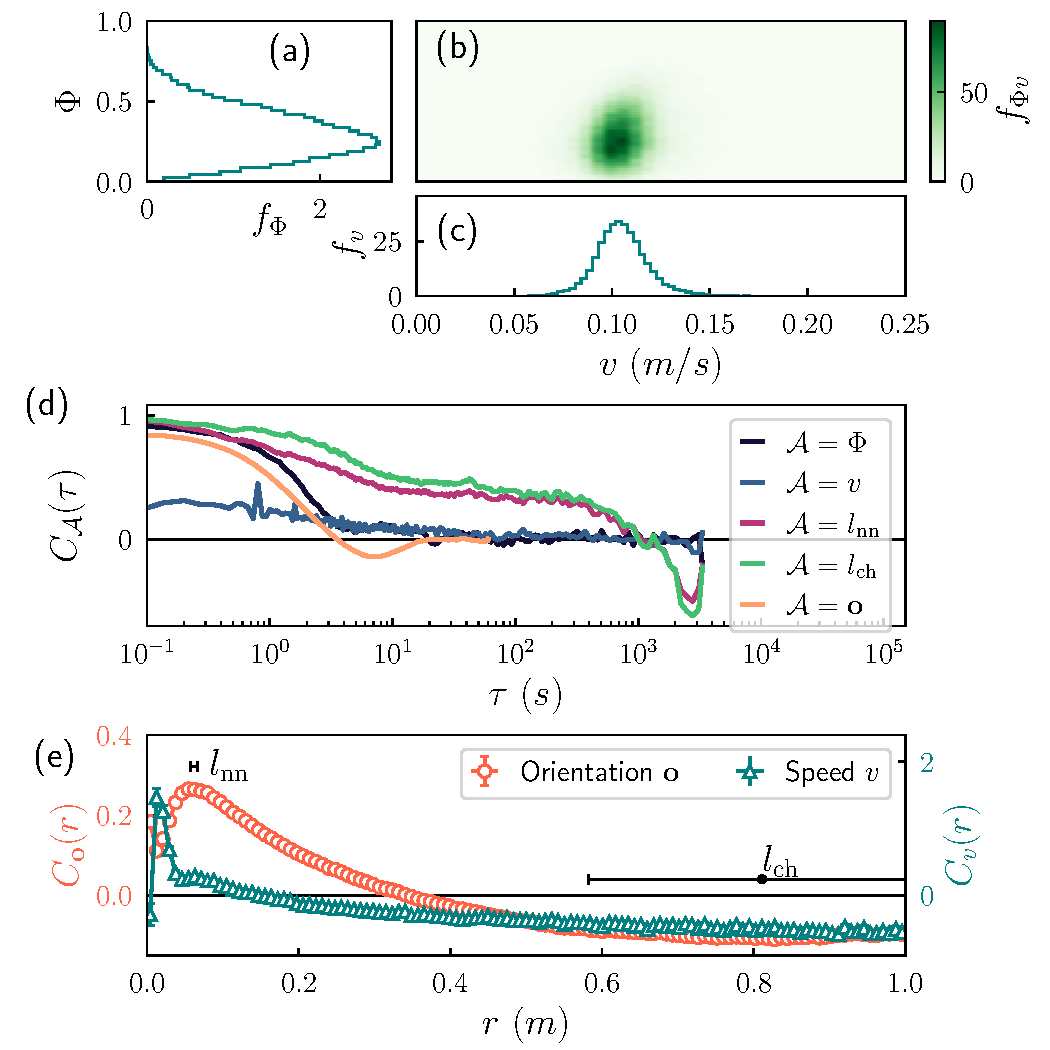
\includegraphics[width=\linewidth]{dynamics-2d-50}
  \caption[The dynamics of 50 fish in 2D]{
  	The dynamics of 50 adult zebrafish in 2D.
  	(a) The probability density function ($f_\Phi$) of the polarisation ($\Phi$, Eq.~\ref{eq:polarisation}).
  	(b) The joint probability density function ($f_{\Phi v}$) for the polarisation ($\Phi$) and the speed ($v$).
  	(c) The probability density function ($f_v$) of the average speed (Eq.~\ref{eq:speed}).
  	(d) The auto-correlation function, $C_\mathcal{A}(\tau)$, of the the polarisation ($\Phi$), the average speed ($v$), the nearest neighbour distance ($l_\mathrm{nn}$), the effective convex hull diameter ($l_\mathrm{ch}$), and the orientation of each fish ($\mathbf{o}$).
  	(e) The connected correlation function of the orientation ($\mathbf{o}$) and speed ($v$), as a function of pairwise distances.
  }
  \label{fig:dynamics-2d}
\end{SCfigure}


On the other hand, the relaxation of the local density, as probed by the ACFs of $l_\mathrm{nn}$ and $l_\mathrm{ch}$, is a much slower process. The two ACFs have two similar relaxation timescales of 900s (15 minutes). This process might corresponds to the fragmentation of the group. As a result, we use this largest timescale ($\tau_\rho \sim$ 900s) to characterise the time it took for 50 zebrafish to forget their state, in a quasi-2D experiment.

The connected correlation function of the fish, for their speed as well as their orientation was plotted in Fig.~\ref{fig:dynamics-2d}(e). Surprisingly, the correlation function of the orientation, $C_\mathbf{o}(r)$, exhibits a much longer correlation length ($\xi_\mathbf{o} \sim 0.38m$), compared to the correlation of the speed ($\xi_v \sim 0.15m$). This picture is very different from European starlings, whose correlations lengths for both orientation and speed were similar \cite{cavagna2010}. Our result suggests the lack of speed synchronisation for the zebrafish, which could be the reason that the fish were always in a randomised state with a low $\Phi$ value.




\subsection{The Changing States}
\label{section:change-states-2d}

Since the fish change their (macroscopic) states in a timescale of 15 minutes, we segment the trajectory into different sections with the duration of 15 minutes. By doing so, we could study the structure and dynamics of the fish as a function of time, since the fish could change their states continuously, rather than being in a steady state.

The changing states of the fish as a function of observation time as plotted in Fig.~\ref{fig:change-states-2d}. The $g(r)$ of the fish were shown in Fig.~\ref{fig:change-states-2d}(a), were the peak of the $g(r)$ gradually decreases with the evolution of time. This suggests a decrease of cohesiveness for the fish group. The ACF of the orientation of the fish, $C_\mathbf{o}(t)$, at different time were plotted in Fig.~\ref{fig:change-states-2d}(b), which exhibit less variation comparing with the $g(r)$ functions.

 \begin{SCfigure}
  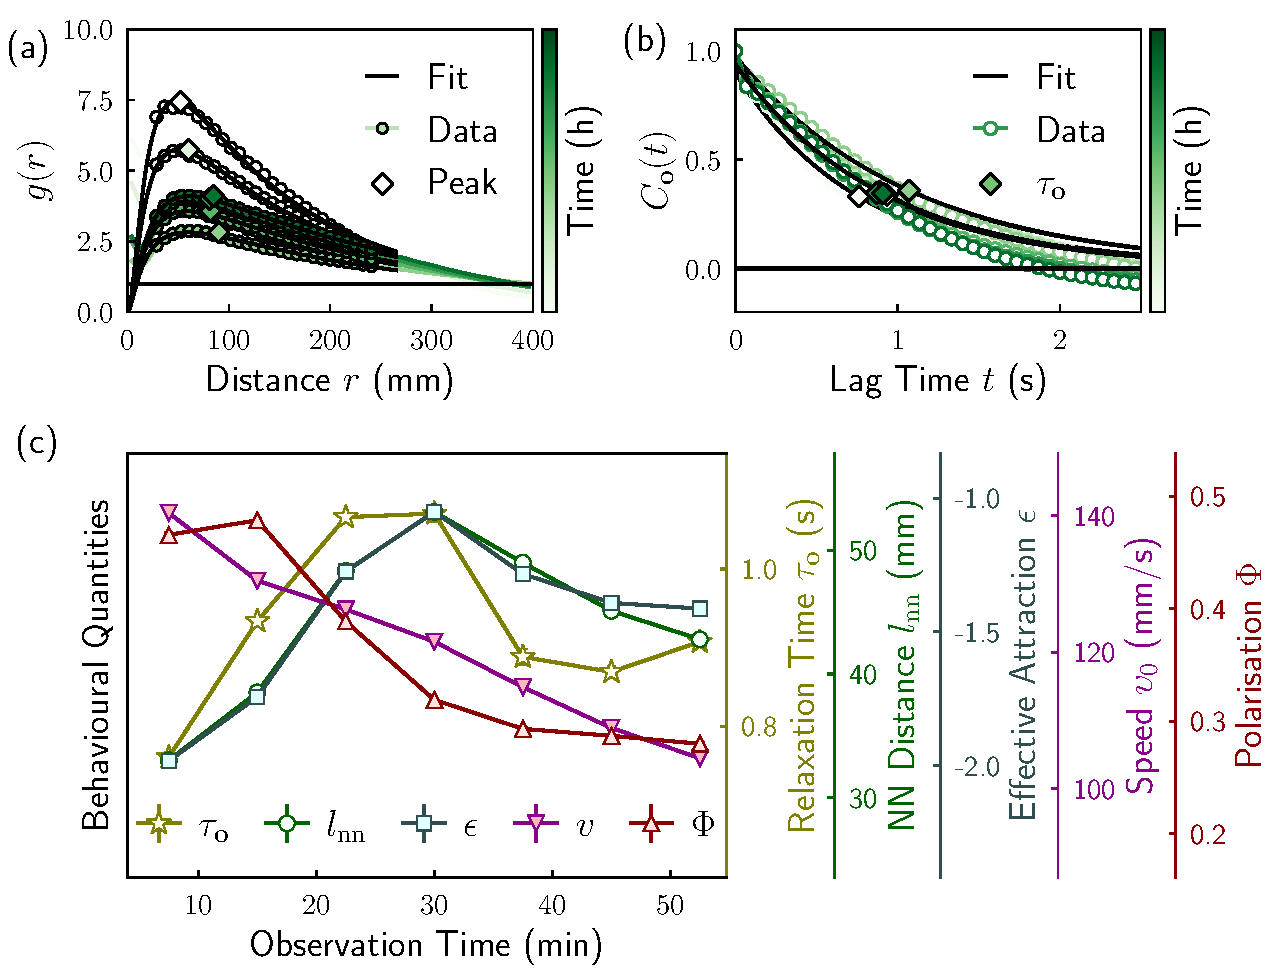
\includegraphics[width=\linewidth,outer]{change-states-2d-50}
  \caption[The changing states of 50 zebrafish in a 2D experiment]{
	(a) Sequence of radial distribution functions, the $g(r)$,  at different time points. In early times (top curves) the fish are clustered together so that the peak is large; at later times (bottom curves) the local density decreases and so does the peak height.
	(b) Sequence of the auto--correlation function of the orientations $C_\mathbf{o}(t)$ of the fish, at different time points.
	(c) The time evolution of the averaged {\descriptors} for 50 {\smallfish} fish. Each point corresponds to the average value in 15 minutes.
	The error bars illustrate the standard error values.
  }
  \label{fig:change-states-2d}
\end{SCfigure}


The time evolution of 5 selected behavioural quantities, the orientational relaxation time ($\tau_\mathbf{o}$, Eq.~\ref{eq:tau}), the nearest neighbour distance ($l_\mathrm{nn}$, Eq.~\ref{eq:nnd}), the effective attraction ($\epsilon$, Eq.~\ref{eq:effective-attraction}), the average speed ($v$, Eq.~\ref{eq:speed}), and the polarisation ($\Phi$, Eq.~\ref{eq:polarisation}), was plotted in Fig.~\ref{fig:change-states-2d}(c). Each point in Fig.~\ref{fig:change-states-2d}(c) corresponds to the time average over 15 minutes. It is clear that the structural quantities ($\epsilon$ and $l_\mathrm{nn}$) were correlated while the dynamical quantities ($v$ and $\Phi$) were correlated.

Surprisingly, the orientational relaxation time seems to correlate with the structural quantities, and the fish exhibit slower orientation relaxation when they were in a less cohesive state. One possible explanation is that the orientation of the fish will be interrupted by a close neighbour, as a consequence of the avoidance for collision. These extra interruptions, on top of the intrinsic orientational diffusion of the fish, make the fish change their orientations faster in a dense group. This picture is also consistence with the observation that the polarisation of the fish increase as the nearest neighbour distances of the fish increase \cite{miller2012}.


\section{The Behaviour of 50 Zebrafish in 3D}

Following the same data processing procedure and analysis, we also studied the behaviour of 50 zebrafish in a 3D observation. In contrast to the 2D experiments where the fish were confined in a shallow water environment, now the fish can explore a 3D space enclosed by the water-air interface and a bowl-shaped tank. The result for one representative 3D experiment will be introduced in this section, while multiple experiments have been repeatedly carried out. The other experimental results will be discussed in section~\ref{section:universal}.

\subsection{The Structure}
\label{section:analysis-structure-3d}


The spatial distribution of 50 zebrafish was shown in Fig.~\ref{fig:structure-3d} (a), where the joint distribution of the $x$ and $z$ coordinate clearly shows the depth preference of the fish, as discussed in section~\ref{section:fish_many_3d}. With the ideal gas sampled according to the distribution of the fish, we calculated the PDF of the pairwise distances, $f_d(r)$, of the fish and the ideal gas. The result is shown in Fig~\ref{fig:structure-3d}(b). It is clear that the fish are more cohesive, as the mode of $f_d^\mathrm{fish}(r)$ locates at a smaller distance value.

The ratio of two PDFs gives the $g(r)$ (Eq.~\ref{eq:gr}), presented in Fig.~\ref{fig:structure-3d}(c). Like the 2D results (Fig.~\ref{fig:structure-2d}), the $g(r)$ exhibits a typical disordered, fluid-like shape, featuring a single peat at $\sim l_\mathrm{nn}$ with a monotonic decay. The height of the peak reaches the value of 5, being larger than the peak height ($\sim 2.2$, Fig.~\ref{fig:structure-2d}(c)) in the 2D experiment. This difference indicates that the 50 fish were swimming in a more cohesive way in the 3D experiment, comparing with the 2D experiment.


Importantly, the correlation length of the density ($\xi_\rho$, Eq.~\ref{eq:length-density}) is close to the effective convex hull diameter ($l_\mathrm{ch}$, Eq.~\ref{eq:convex-hull-diameter}), as shown in Fig.~\ref{fig:structure-3d}. This suggests the fish remained a compact, and cohesive group in the 3D experiment. A snapshot of such a cohesive group was plotted as circular markers in Fig.~\ref{fig:structure-3d} (a).

Since the fish always form a compact cluster, a cohesive clique, when they were swimming in the 3D observation tank, there is no void in the length scale of the convex hull of the group. Comparing with the size of the explorable environment, the $l_\mathrm{ch}$ is mush smaller, and the void corresponds to the space where the fish aggregation could explore collectively.

The cohesive nature of the fish in the 3D experiment is also supported by the distribution of the $l_\mathrm{ch}$ shown in Fig.~\ref{fig:structure-3d}, which is much narrower than that from the 2D experiments. Interestingly, the distribution of $l_\mathrm{nn}$ for the fish swimming in both 3D and 2D environments were close. Numerically, the averaged $l_\mathrm{nn}$ value for the 3D experiments were slightly smaller than the value from 2D experiments (Table~\ref{table:behaviour}).


\begin{SCfigure}
  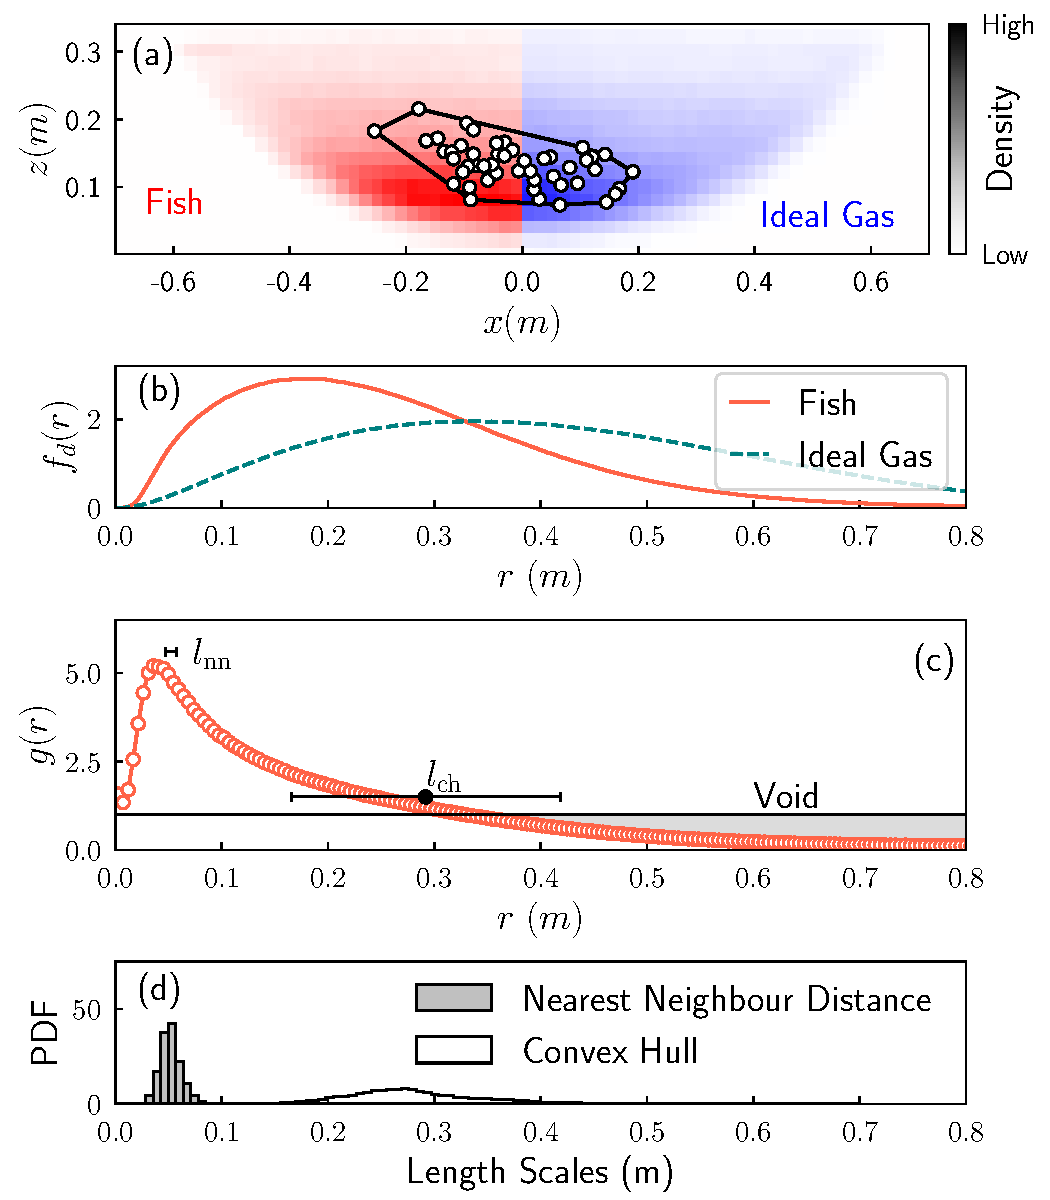
\includegraphics[width=\linewidth]{structure-3d-50}
  \caption[The structure of 50 fish in 3D]{
  	The structure of 50 adult zebrafish in 3D.
  	(a) The joint distribution of the $x$ and $z$ coordinates of the fish and the ideal gas particles. The distribution of the ideal gas is biased to be identical to the fish. The location of 50 fish at one time point is plotted as circles. The boundary convex hull of these 50 scatters is plotted as solid lines.
  	(b) The probability density function of the pairwise distributions for the fish and the ideal gas particles.
  	(c) The radial distribution function, $g(r)$ (Eq.~\ref{eq:gr}) of the fish. It is defined as the ratio between the two PDFs in (b). Two important length scales, the nearest neighbour distance and the size of the convex hull were captured by the $g(r)$. The long distance region where $g(r) < 1$ corresponds to the void in the tank, where the group were able to explore.
  	(d) The distribution of the nearest neighbour distance and the effective diameter of the convex hull, of the fish.
  }
  \label{fig:structure-3d}
\end{SCfigure}

\subsection{The Dynamics}


The dynamics of the 50 zebrafish in a 3D observation experiment is shown in Fig.~\ref{fig:dynamics-3d}. Figure~\ref{fig:dynamics-3d} (a)-(c) shows the distribution of the speed ($v$) and the polarisation ($\Phi$), as well as the joint distribution of the two. Interestingly, the speed exhibits a bimodal distribution (Fig.~\ref{fig:dynamics-3d}), indicating the fish were changing between a slow state to a fast state during the observation. The joint PDF of $v$ and $\Phi$ exhibits a positive correlation, as shown in Fig.~\ref{fig:dynamics-3d}(b).


The ACF of different structural quantities and dynamical quantities for 50 fish were plotted in Fig.~\ref{fig:dynamics-3d}(d). Like the 2D results, these ACFs exhibit two decays, featuring the relaxation of the orientation ($\tau_\mathbf{o} \sim 1s$) and the local density ($\tau_\rho \sim 120s$). The latter timescale is used to separate the observation into separate segments, to study the time evolution of the fish states in section~\ref{section:change-states-3d}.


\begin{SCfigure}
  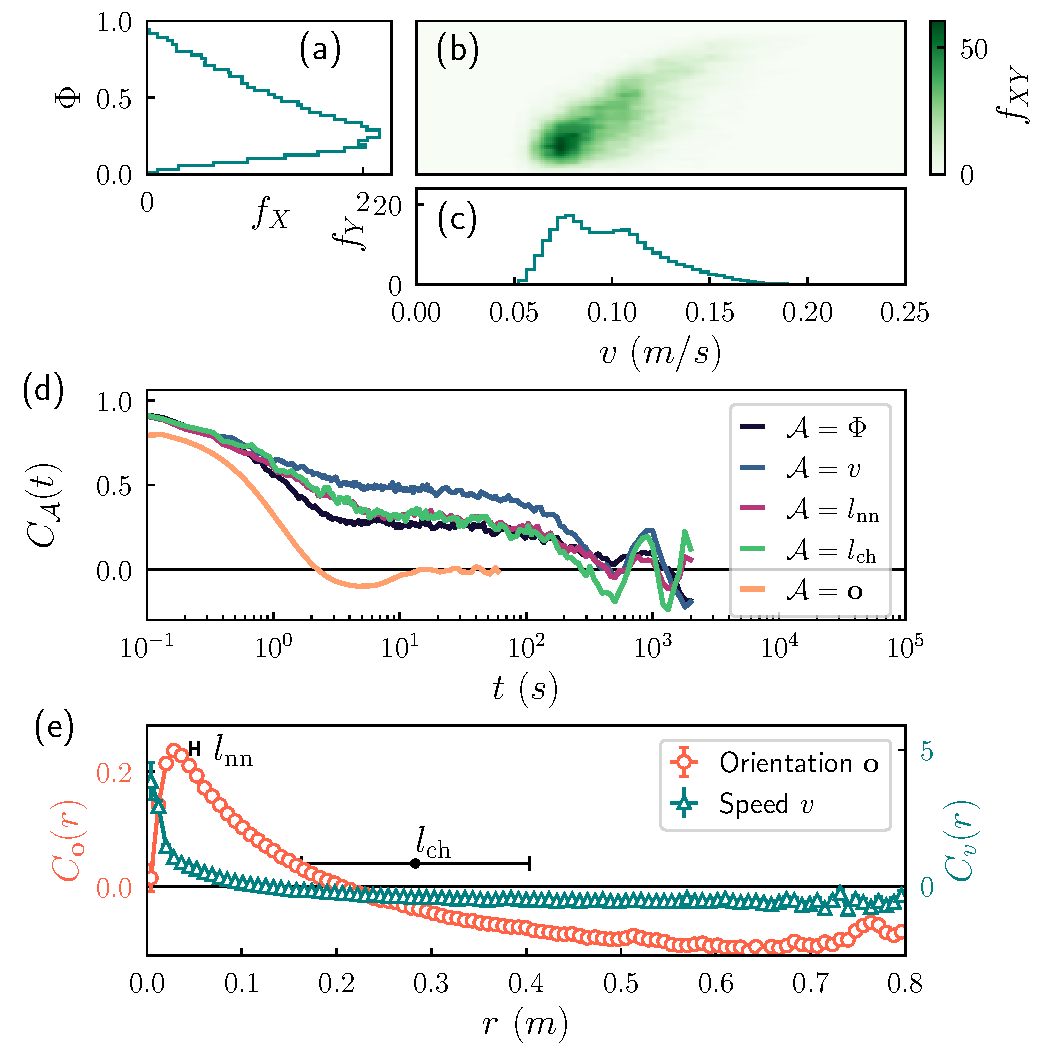
\includegraphics[width=\linewidth]{dynamics-3d-50}
  \caption[The dynamics of 50 fish in 3D]{
  	The dynamics of 50 adult zebrafish in 3D.
  	(a) The probability density function ($f_\Phi$) of the polarisation ($\Phi$, Eq.~\ref{eq:polarisation}).
  	(b) The joint probability density function ($f_{\Phi v}$) for the polarisation ($\Phi$) and the speed ($v$).
  	(c) The probability density function ($f_v$) of the average speed (Eq.~\ref{eq:speed}).
  	(d) The auto-correlation function, $C_\mathcal{A}(\tau)$, of the the polarisation ($\Phi$), the average speed ($v$), the nearest neighbour distance ($l_\mathrm{nn}$), the effective convex hull diameter ($l_\mathrm{ch}$), and the orientation of each fish ($\mathbf{o}$).
  	(e) The connected correlation function of the orientation ($\mathbf{o}$) and speed ($v$), as a function of pairwise distances.
  }
  \label{fig:dynamics-3d}
\end{SCfigure}


The connected correlation function of the speed and orientation of the fish, $C_v(r)$ and $C_\mathbf{o}(r)$, was presented in Fig.~\ref{fig:dynamics-3d}(e). Being very similar to the 2D results, the orientation of the fish exhibits a longer correlation length compared with the speed. The two correlation length values, $\xi_\mathbf{o}$ and $\xi_v$, are listed in Table~\ref{table:behaviour}.

Comparing with the 2D results in Fig.~\ref{fig:dynamics-2d}, the fish were swimming at a similar speed in a 3D environment, with $v_\mathrm{2D} = 0.11m/s$ and $v_\mathrm{3D} = 0.098m/s$. However, the fish were swimming in a more ordered way in a 3D observation, indicated by the high $\Phi$ values at the tail of the distribution $f_\Phi$. 
It is notable that the ACFs of the structural quantities ($l_\mathrm{nn}$ and $l_\mathrm{ch}$) and dynamical quantities ($\Phi$ and $v$) sharing the same shape for the fish in the 3D observation. This similarity of the ACFs was not observed in the 2D experiments.

%The fact that the fish presents different behaviour with varying degrees of order was also observed by \citeauthor{miller2012}, where the movement of zebrafish changed from ordered to disordered over time \cite{miller2012}.


\subsection{The Changing States}
\label{section:change-states-3d}

\begin{SCfigure}
  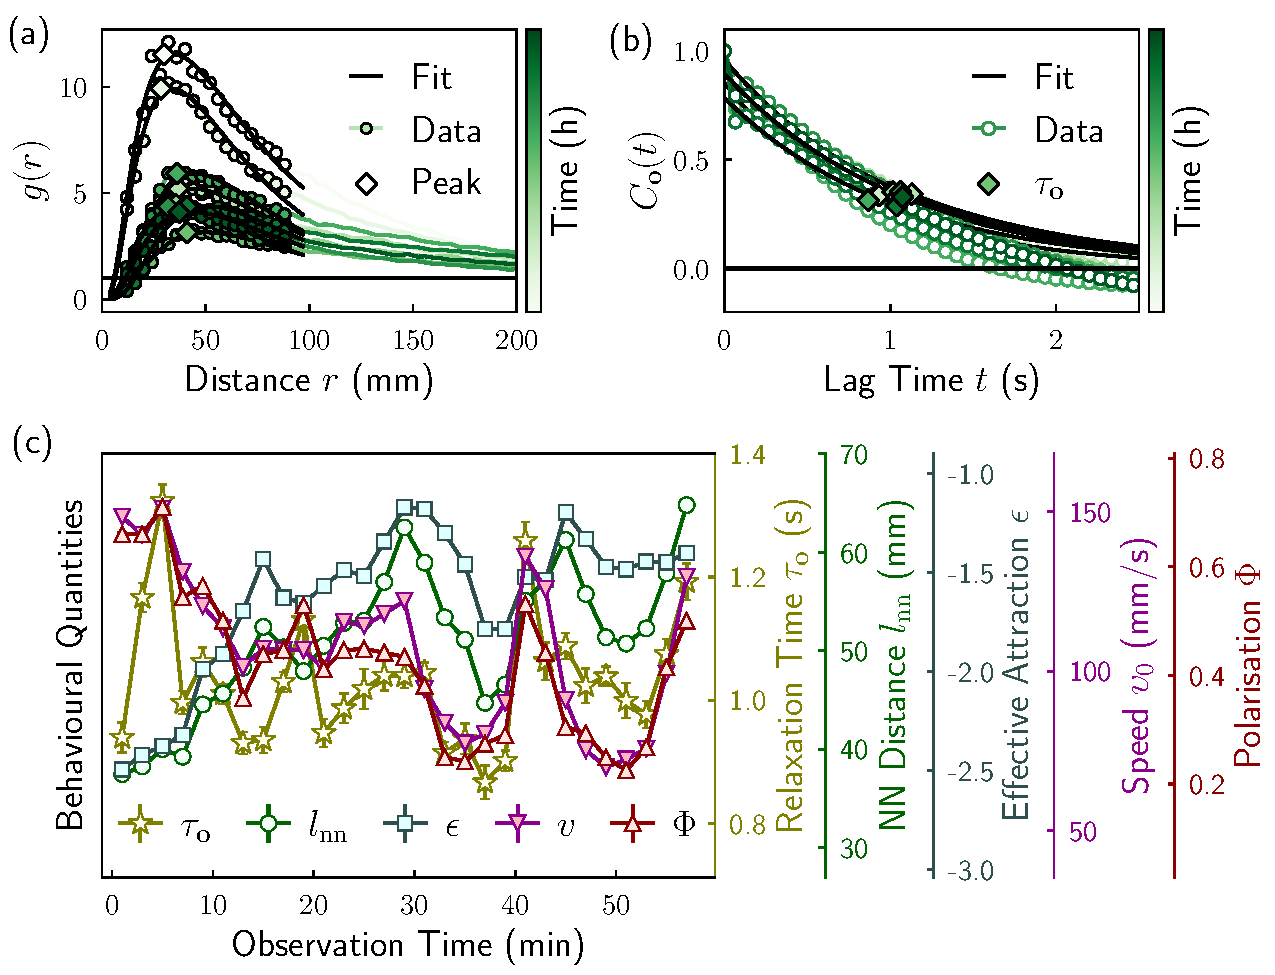
\includegraphics[width=\linewidth,outer]{change-states-3d-50}
  \caption[The changing states of 50 zebrafish in a 3D experiment]{
	(a) Sequence of radial distribution functions, the $g(r)$,  at different time points. In early times (top curves) the fish are clustered together so that the peak is large; at later times (bottom curves) the local density decreases and so does the peak height.
	(b) Sequence of the auto--correlation function of the orientations $C_\mathbf{o}(t)$ of the fish, at different time points.
	(c) The time evolution of the averaged {\descriptors} for 50 {\smallfish} fish. Each point corresponds to the average value in 2 minutes.
	The error bars illustrate the standard error values.
  }
  \label{fig:change-states-3d}
\end{SCfigure}

To study the changing states of the fish group, we separated the observation into short segments of 120s, and analyse the behaviour of the fish in these short periods separately. The results are shown in Fig.~\ref{fig:change-states-3d}. 
For each segment, we calculated the ACF of the orientation, as shown in Fig.~\ref{fig:change-states-3d} (b), as well as the $g(r)$, plotted in Fig.~\ref{fig:change-states-3d}(a). From these two correlation functions, we extracted the changing $\tau_\mathbf{o}$ and the changing effective attraction ($\epsilon$) values. Like the behaviour of fish during our 2D observation, the cohesion among the fish gradually decreases, indicated by the decreasing height of the peak in the $g(r)$. However, no systematic change of the $C_\mathbf{o}(t)$ were observed.

The time evolution of different structural and dynamical quantities were plotted in Fig.~\ref{fig:change-states-3d}(c). All these quantities change with time, indicating the fish were constantly changing their states.
The speed is correlated with the polarisation, and the nearest neighbour distance is correlated with the effective attraction.


These correlations were also observed from our 2D experiments in Fig.~\ref{fig:change-states-2d}. The non-linear nature of the time-evolution of fish states revealed the complexity of the behaviour of the fish, and more controlled experiments is necessary to differentiate the possible origins, that are responsible for the changing states of the fish. For instance, a sudden noise in the environment might trigger the jump in speed in Fig.~\ref{fig:change-states-3d}. But such change, termed as the spontaneous startle cascades in \cite{rosenthal2015}, might also emerge naturally without any triggering factor. Unfortunately, the exact cause of these sudden changes is unknown\marginfootnote{
Ideally, I should monitor the noise level and the vibrations of the water in the tank, to study if they affect the fish behaviour or not. However, the relevant data was not recorded. Practically, the experimental setup was located in a relatively quiet room. Closing the door of a nearby room would make a noticeable noise, whose effect on the fish behaviour is unknown.
}.



\section{The Universal Behaviour of Zebrafish}
\label{section:universal}


The complicated changing states of the fish shown in Figs.~\ref{fig:change-states-2d} and \ref{fig:change-states-3d}, can be captured by one number, regardless of the dimension of the swimming environment. This number is termed as the \emph{reduced persistence length} (\gls{kappa}), whose definition is,

\begin{equation}
	\kappa 
	= \frac{v \tau_\mathrm{o}}{l_\mathrm{nn}}
	= \frac{l_p}{l_\mathrm{nn}}	.
\label{eq:kappa}
\end{equation}

\noindent The value of $\kappa$ correlates robustly with the value of polarisation $\Phi$, as shown in Fig.~\ref{fig:states-1d}.
This correlation is remarkable because it describes all the experimental observations on different adult zebrafish groups, with different ages.
%This robust correlation is the most important result in this thesis.
A very simple argument for the correlation is that each fish could share its current moving direction with the group, in the lengthscale of $l_p$. Such information could be transmitted to more members in a cohesive group, with smaller $l_\mathrm{nn}$ value. When more members were exchanging their information about the moving direction, the entire group is more likely to form a consensus, and exhibit ordered movement with a high $\Phi$ value.

This explanation is helpful because it relates the property of the individual fish (the persistence length, and the local density) to the macroscopic behaviour (the polarisation).
Such connection is vital to understand the behaviour of mutant zebrafish, which had significantly larger $l_p$ values comparing with the wildtype zebrafish. The relevant results will be presented in chapter~\ref{chapter:fish_mutation}.
In addition, it is easy to compare the observed experimental result in Fig.~\ref{fig:states-1d} with the computer simulations of agent-based models, since both $\kappa$ and $\Phi$ are dimensionless numbers. Such comparison will be discussed in chapter~\ref{chapter:fish_model}.


 \begin{SCfigure}
  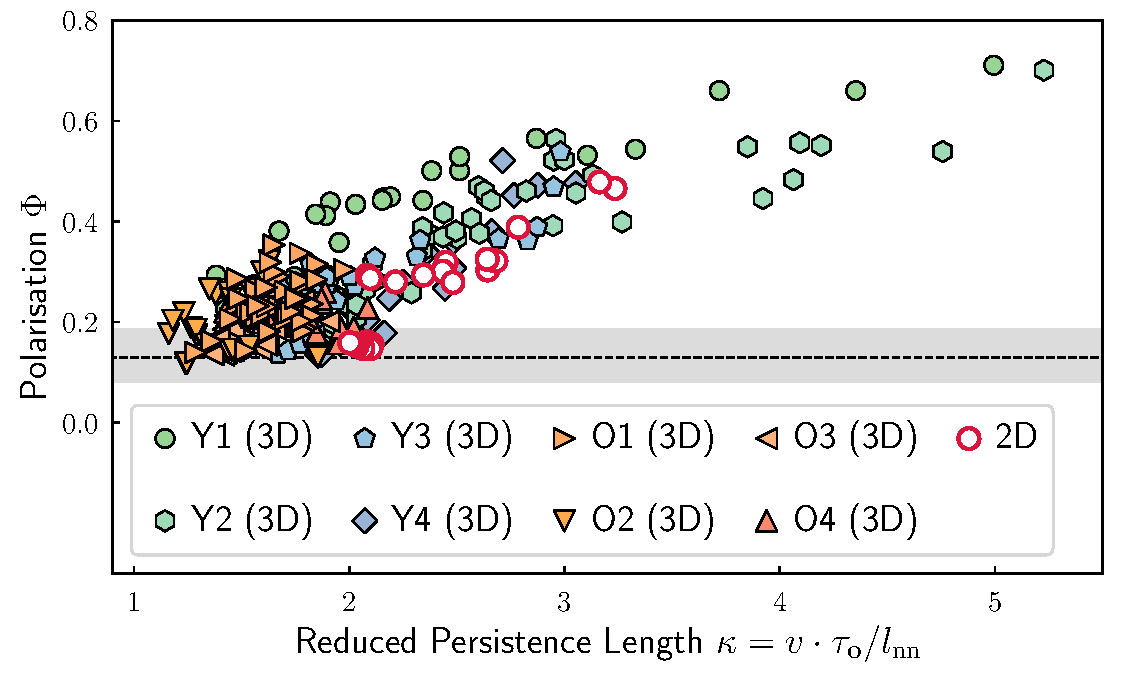
\includegraphics[width=\linewidth,outer]{states-1d}
  \caption[The behaviour of 50 zebrafish described by reduced persistence length]{
  	The relationship between the polarisation, the order of the movement, and the reduced persistence length of the fish. For the 3D observation, multiple repeated measurement with different fish groups at different dates were collected (Y1-Y4: different young fish groups; O1-O4: different old fish groups).
  	All of the observed fish behaviour results were collapsed onto a master curve. The result of one 2D observation was also included, as open circles. The 2D results does not collapse onto the same master curve from the 3D data, because of the difference in the dimensions.
  }
  \label{fig:states-1d}
\end{SCfigure}

\vfill
\pagebreak

\begin{adjustwidth}{-5cm}{0cm}
\begin{tcolorbox}[
fonttitle=\sffamily\Large,
right=0.05\linewidth,
title=Summary of Chapter~5
]
\begin{itemize}
	\item We discussed the methods to analyse the experimental coordinates of the zebrafish, in order to study their collective behaviour. There are four steps.
	\begin{description}
		\item[1. Refining Coordinates] \hfill \\
		Some coordinates are very close to each other, which are physically impossible. These overlapping particles can be removed with an optimisation algorithm.
		\item[2. Linking Coordinates into Trajectories] \hfill \\
		The refined coordinates can be linked into trajectories, and the short trajectories can be extended using methods in section~\ref{section:link}.
		\item[3. Analysing the Structure of the Fish Group] \hfill \\
		We use the nearest neighbour distance ($l_\mathrm{nn}$), the size of the convex hull ($l_\mathrm{ch}$), and the radial distribution function $g(r)$ to characterise the structure of the fish group.
		\item[4. Analysing the Dynamics of the Fish Group] \hfill \\
		We use the average speed ($v$), the polarisation ($\Phi$), the relaxation time scales ($\tau$) to characterise the dynamics of the fish group.
		In addition, we use the correlation functions of the orientation and the speed, $C_\mathbf{o}(r)$ and $C_v(r)$, to measure the dynamical lengthscales.
		\end{description}
	\item We get the following results from the 2D movement of 50 zebrafish.
	\begin{itemize}
		\item The fish groups segmented into sub-clusters.
		\item The fish groups were in the disorder phase, with low polarisation values.
		\item The collective motion of the fish groups exhibited a short time scale related to the reorientation of the fish individual (1 s), and a large time scale related to the relaxation of the local density (15 minutes).
		\item The correlation length of orientation is longer than the correlation length of the speed.
		\item The macroscopic state of the fish group changes over time, indicated by the changing quantities in Fig.~\ref{fig:change-states-2d}.
	\end{itemize}
	\item  We get the following results from the 3D movement of 50 zebrafish.
	\begin{itemize}
		\item The fish group remained a cohesive cluster without fragmentation.
		\item The fish group switched between the ordered phase and the disorder phase, with varying polarisation values.
		\item The collective motion of the fish group exhibit a short time scale related to the reorientation of the fish individual (1 s), and a large time scale related to the relaxation of the local density (2 minutes).
		\item The correlation length of orientation is larger than the correlation length of the speed.
		\item The macroscopic state of the fish group changes over time, indicated by the changing quantities in Fig.~\ref{fig:change-states-3d}.
	\end{itemize}
	\item The change of the macroscopic states of the zebrafish groups is not totally random. The ratio between the persistence length and the nearest neighbour distance, for both 2D and 3D data, presents a robust correlation with the polarisation. The fact, that similar conclusions were reached from 2D and 3D experiments, is in accordance with previous studies \cite{watts2017, romenskyy2020}.
\end{itemize}
\end{tcolorbox}
\end{adjustwidth}


\end{document}
